\chapter{Designing X-ray Visualizations with Volume Rendering} \label{Chap:VolumetricX-rayVision}
% Introduction to this section: why is this chapter required
This chapter presents an investigation into the use of volume rendering to support \glspl{X-ray Visualization} by providing an explanation of the technical aspects of volume rendering and motivating the opportunity of volume rendering. 
Then, it presents a summary of volume rendering techniques and algorithms designed and demonstrated for use on stereoscopic displays, which form the basis of the research in this dissertation.
Finally, drawing from the knowledge from the literature review (\autoref{chap:Background}) and the previous study (\autoref{Chap:X-ray Implemntion}) to create a new form of X-ray Visualizations the \glspl{virt}.


% Firstly, we will provide a grounding for the unlying technology that the X-ray visualizations being tested in this study will use.
The \glspl{virt} are designed for \gls{mri} and \gls{ct} data when displayed using \gls{dvr} and how to view the inside of a solid object that they are captured from.
The image data from \gls{mri} and \gls{ct} scanners has been chosen as the main focus as these devices are the most commonly used forms of volume rendering that are used to look inside of objects rather than trying to visualize or make other data readable.

%These techniques can likely be extended to other uses for \gls{dvr} as they all utilize a similar geometrical space.
%two methods into something were brought up. One of them would be to place cameras behind the real world and create a scene, which does not work well when you can not access the inside of the object.
% Causes this chapter to focus on creating X-ray visualizations that you can see into.

\begin{figure}[tb]
    \centering
    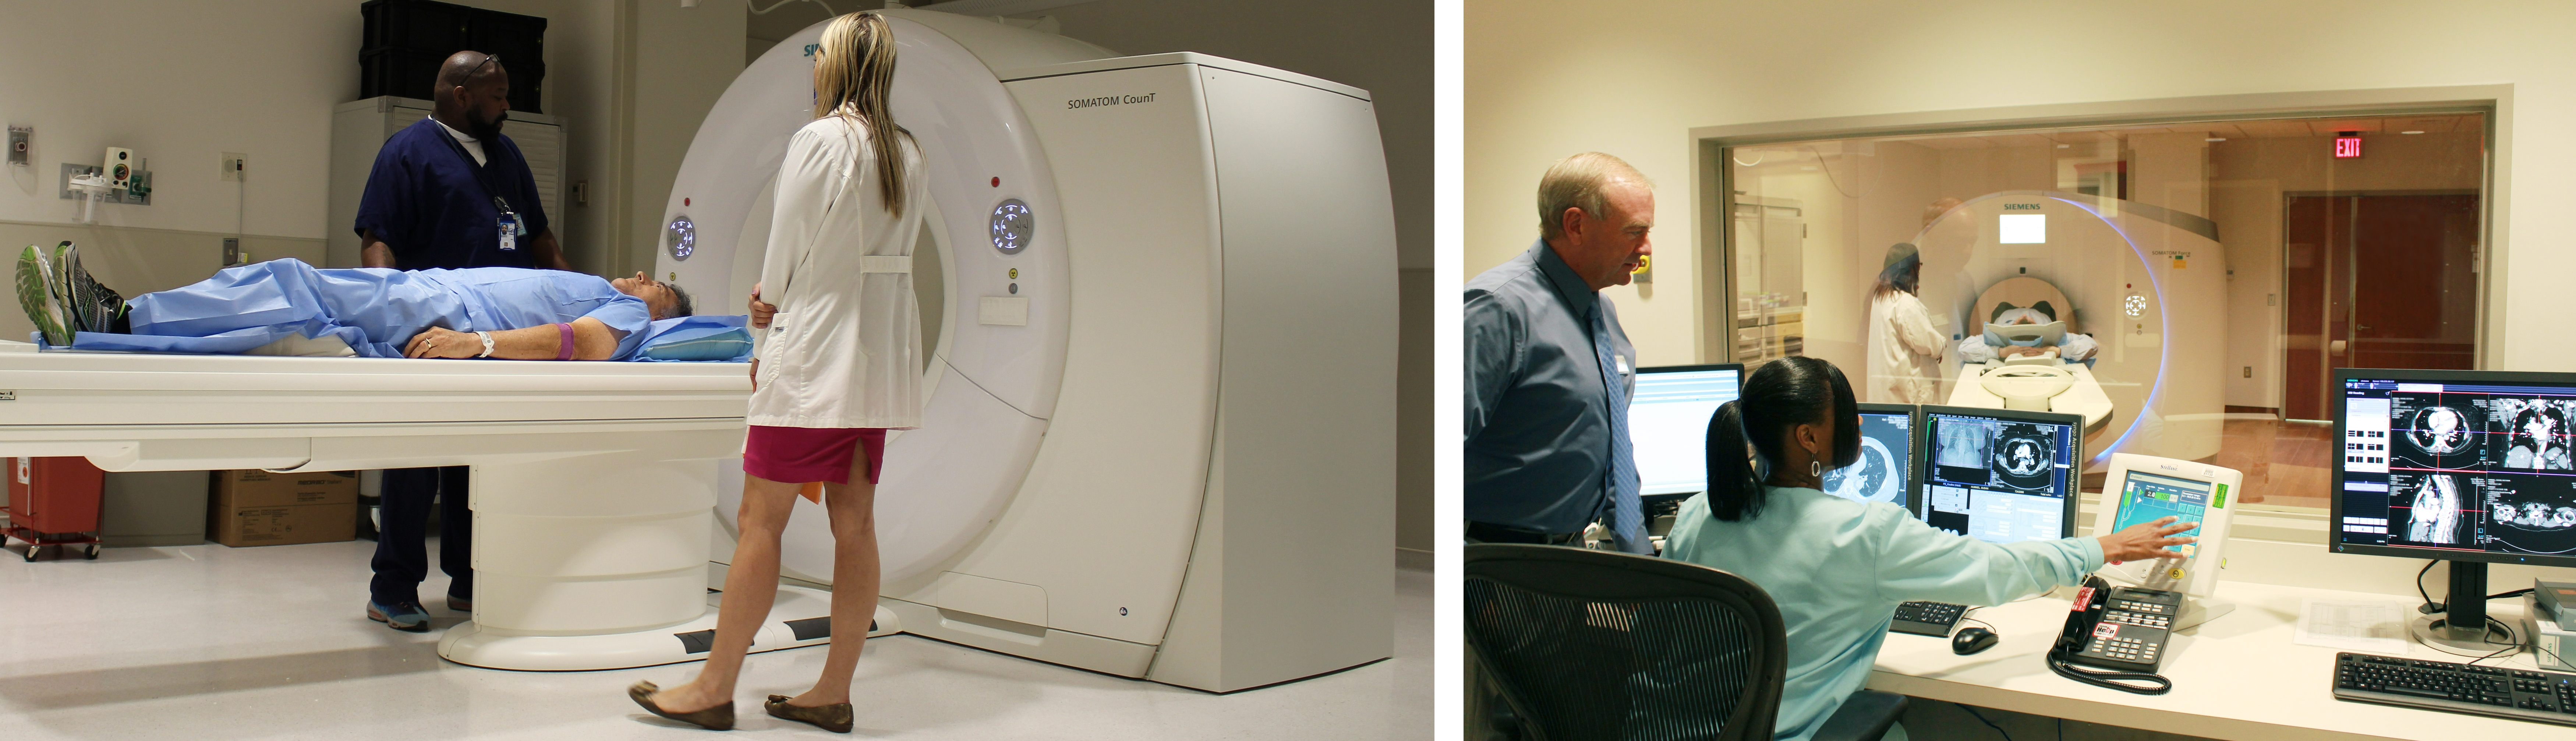
\includegraphics[width=\linewidth]{Chapter4/Images/CTScannersCropped.jpg}
    \caption[A patient receiving a scan in the \gls{ct} scanner]{A patient receiving a scan in the \gls{ct} scanner. Left) shows the environment within the Scanning Room. Right) is one example of an operation area for a given \gls{ct} scanner. Provided by NIH Clinical Center}
    \label{fig:CTScanner}
\end{figure}


To understand what is inside solid objects, a 3D scanning technique will need to be utilized, allowing people to observe an area using a method that human sight can use.
Some options exist for the creation of this volume rendering data. 
Firstly, they can be created manually or from the result of a simulation~\cite{Avila1994} or by using other solutions like tracking the speed of signals between different areas~\cite{Adib2013}.
Electronic microscopes can visualize the data they see as a volume~\cite{Goodsell1989, Khlebnikov2013}.
\gls{gpr} can be used to understand what is below the ground, from pipes and artifacts to different layers of ground sediments~\cite{Maloca2018, VanSon2018, Baker2007}.
\gls{mri} and \gls{ct} scanners are more commonly used to see the inside of people~\cite{Alhazmi2018, Zhang2011} and most other types of materials~\cite{Okuyan2014, Groger2022, Vicente17}.

% DataFromScans.png
\begin{figure}[tb]
    \centering
    \includegraphics[width=\linewidth]{Chapter4/Images/DataFromScans.png}
    \caption[Left) \gls{mri} of a skull; Center) Cerebral angiography, arteria vertebralis sinister injection; Right) CT scan of human lungs.]{
    Several different types of 2D data: 
    Left) \gls{mri} of a skull~\footnotemark[1];
    Center) Cerebral angiography, arteria vertebralis sinister injection~\footnotemark[2];
    Right) CT scan of human lungs~\footnotemark[3].
    All images are licensed under Creative Commons Attribution licences}
    \label{fig:CTScans}
\end{figure}

\footnotetext[1]{\url{https://www.flickr.com/photos/reighleblanc/3854685038}}
\footnotetext[2]{\url{https://en.m.wikipedia.org/wiki/File:Cerebral\textunderscore angiography,\textunderscore arteria\textunderscore vertebralis\textunderscore sinister\textunderscore injection.JPG}}
\footnotetext[3]{\url{https://commons.wikimedia.org/wiki/File:CT\textunderscore scan\textunderscore Iterative\textunderscore reconstruction\textunderscore \%28left\%29\textunderscore versus\textunderscore filtered\textunderscore backprojection\textunderscore \%28right\%29.jpg}}
% provides a high-level description of what the term volume rendering encapsulates (2 - 3 paragraphs)
Medical practitioners' current practice is to view medical data on a 2D display near the patient. 
This is shown in \autoref{fig:CTScanner} where the practitioner is in a separate room with a window between them and the patient looking at a series of slices from the scan.
Their concentration will be on this display, which will display images shown in \autoref{fig:CTScans}, where they can view the data from a series of 2D planes of view (axial, coronal, and sagittal). 
This type of exploration can be challenging to learn and interpret methods of data interaction~\cite{Brath2015, Vernon2002, Tang2019}.
The experience on 3D displays can be better suited for viewing 3D data~\cite{McIntire2012, Merino2018, Thomas2015}, and studies have shown that displaying this data over real objects can further aid this understanding~\cite{Martin-Gomez2021, Pratt2018, Fischer2020}. 
This makes volume rendering more suitable for \gls{mr} \glspl{hmd} as they utilize 3D displays. 
%This better experience still needs to be understood to place the internal data in the place it was pictured~\cite{Martin-Gomez2021, Pratt2018, Fischer2020}.

% To talk about issues in this field regarding testing
%This thesis focuses on looking into objects you usually could not and how this is best handled.
%We typically utilize \gls{mri} and \gls{ct} scanners to investigate areas inside of objects that we could not usually; however, this experience is not simple to deal with. 
\gls{mri} and \gls{ct} scanners are utilized to investigate areas inside objects that could not usually be seen; however, this experience is not simple.
%\gls{dvr} visualizations are suitable for hole-like X-ray visualizations since they naturally utilize the same geographic methods required.
Hole-like visualizations work by obscuring most of the data collected, which is required to create the \gls{X-ray Vision} effect. 
This is problematic as \gls{mri} and \gls{ct} scans generally only observe the immediate area.
Since they only show three axes, the only logical forms of entry are along the three planes (axial, coronal, and sagittal)~\cite{Joshi2013}.
3D objects also allow for navigating challenging anatomy that can take on multiple different shapes, like the liver~\cite{DePaolis2018}.

The radiation caused by \gls{ct} scanners can be harmful to the health of patients. Both \gls{mri} and \gls{ct} scans are time-consuming and expensive, limiting the amount of data that can be realistically collected when medical practitioners produce the \gls{mri} or \gls{ct} scans designed to diagnose and guide appropriate treatment.
This will generally result in a trade-off between the size and accuracy of the volumes these machines create. 
Since this supply is already limited, using a method of \gls{X-ray Vision} that requires excess information to be provided to adequately a hole-like \gls{X-ray Vision} technique in practice would require a change in best practice to collect more data, which would just be used to aid the illusion of depth perception. 
%The x-ray visualizations (the \glspl{virt}) avoid these issues and can be used without major changes to the current practices.

% % Methods that work for using this type of visualization to create \gls{X-ray Vision} effects
% Medical practitioners produce and create the \gls{mri} or \gls{ct} scans designed to diagnose and guide appropriate treatment.
% This is generally because there will need to be a trade-off between the size and accuracy of the volumes these machines create. 
% After all, the time required for these machines is valuable. Even though \gls{ct} scanners are faster, they also emit radiation, potentially harming the patient if the exposure lasts too long. 
% What is needed is an \gls{X-ray Vision} method that can be utilized for \gls{dvr}; it is important to consider the environment that can be made and used without major changes to the current workload.

This chapter aims to enable methods of \gls{X-ray Vision} that can be used with \gls{dvr} to create a method to view information created from \gls{mri} or \gls{ct} scanners using an \gls{ost} \gls{ar} \gls{hmd}.
This will utilize artistic effects (\glspl{virt}) because they do not obscure the focus of the user while still presenting the illusion of depth within the real world. 
However, before that goal is reached, there is a need to create and establish a method of real-time \gls{dvr} for stereoscopic displays. 
This chapter presents a novel apparatus to employ DVR on MR, allowing \glspl{virt} to be presented to users.

% Taling about the types of visualizations explored in this part of the paper.
% This Chapter discusses several \gls{X-ray Vision} types in \autoref{chap:Background}. 
% There are generally two methods of seeing things from other fields. 
% One would be placing cameras behind the real world, allowing for \gls{X-ray Vision}, or creating a scene on the other end by reconstructing the images or medical imaging devices. 
% This thesis will focus on the latter and look at how data from MRI or CT scanners can deliver \gls{X-ray Vision} for OST AR devices, which do not obscure any information but allow for a similar effect of \gls{X-ray Vision}. 

\section{Fundamentals of Volume Rendering}
%The volume dataset has some expectations. 
Volume datasets represent information relating to a given physical space~\cite{Kaufman2005}. 
They can either be viewed as a stack of 2D images, a singular 3D image, or a vector or scalar field. 
Volume datasets are known for representing \gls{ct} and \gls{mri}, but they are also used for displaying geometric data that consists of information that can be described in a voluminous way, such as meteorological data~\cite{Kaufman2005, Joshi2009}. 

\subsection{Technical Description of Volume Rendering}
Volumes are organized into a grid of \glspl{voxel_g}, each with its own position and value. 
These values can range in their purpose from Houndsvile units found in \gls{ct} scans~\cite{DenOtter2024}, relaxation times for \gls{mri} scans~\cite{Rinck2024}, and they can either contain normals or velocity when looking at such as meteorological data~\cite{Joshi2009}. 
Generally, a default value is chosen when no value exists in a particular area.
This makes volume data much less flexible than point cloud data but allows for more flexibility with the rendering process. 

Volumes can also be extended into having a fourth dimension, which will normally represent time, allowing them to change the visualization based on the amount of time that has passed. 
This can be used in medicine to give the surgeon a clear idea about how much organs in a patient may move normally~\cite{Langner2008, Gill2015} or to allow meteorologists to view the impact of phenomena like wind in real-time~\cite{Wang2018, HibbardL.1986}. 

\subsection{Visualizing Volume Data}
% Explaining quickly how rendering is usually done
To visualize a volume in 3D, it is preprocessed into an iso-surface or rendered directly. 
Creating an iso-surface makes it possible to use more traditional graphical rendering methods to visualize the volume, allowing these visualizations to be viewed using less computationally expensive at run time~\cite{Baoquan2016, Lorensen}.
Lowering the resulting polygon count of these volumes makes it possible to allow them to work on even less powered devices~\cite{Newman2006}.
However, preprocessing a volume into an iso-surface requires running time-consuming processes, which decreases and warps the amount of information seen. 
Typically, this type of visualization will be used to see only a few different surfaces of the volume~\cite{Newman2006}.
Showing multiple surfaces transparently also causes similar issues to traditional rendering, where an object is not entirely in front of or behind, and another transparent object is not.
When accurate results are required or when dealing with complex structures, \gls{dvr} is a more practical choice because it provides additional information that can be filtered in real time~\cite{Dai2021}.

\subsection{Direct Volume Rendering (DVR)}
% Start Talking about DVR
\gls{dvr} directly renders the data from the volume and displays it as a 3D image.
This allows for realistic images like those shown in \autoref{fig:CinimaticRendering}, which are accurate to the source with very low preprocessing costs, which consist of reading in the files to the \gls{gpu}.
\gls{dvr} has the drawback that it is slow to render with the images in  \autoref{fig:CinimaticRendering}, taking over 3 minutes to render~\cite{Eid2017}. 

An advantage to \gls{dvr} is that it provides a very flexible framework for rendering. 
It is capable of allowing versions of \gls{dvr} to focus on making the best image possible and others to focus on providing smooth interactions on lower-powered devices~\cite{Li2003, Morrical2019, Hadwiger2018, Deakin2019}. 
\gls{dvr} has many methods to make it work efficiently on mobile devices, with several recent studies getting \gls{dvr} to work on the HoloLens 1 and 2~\footnote{\url{https://www.microsoft.com/en-au/hololens}}~\cite{Jung2022, Cetinsaya2020}.

\subsection{Light Simulation Using Direct Volume Rendering}
Generally, \gls{dvr} simulates rays of light that travel through the volume.
Mathematically, moving along a given ray is the same even when working with non-light-based visualizations, such as determining the direction of wind from meteorological data.

These photons will traverse times across different distances in each render. 
When the photon collides with a value, several outcomes can occur. 
These can be categorized as Absorption, Out-Scattering, Emission, and In-Scattering.
Absorption characterizes the radiance of a given field, while emission is a separate radiance field that calculates the radiance added to the field. 

The collision between the ray or photons triggers light propagation and determines how much radiance can be seen throughout a volume~\cite{Chandrasekhar1950}. 
Any form of volume rendering can provide some form of absorption and emission of light. 
Absorption and emission methods are regularly used in real-time volume rendering as they are computationally inexpensive~\cite{Fong2017}. 
Scattering describes the phenomenon where light is deflected in different directions as it interacts with particles within the medium.
Scattering is computationally expensive, requires more computing power, and can be provided in real time. 

Even only utilizing one of these techniques can allow for some form of display using volume rendering, and since they can take drastically different amounts of time. 
This results in two different mechanisms for using DVRs. One of them is real-time, where a user interacts with and manipulates the display in real-time and moves around it. 
This version of \gls{dvr} can be utilized using \gls{mr} devices~\cite{Jung2022, TUKORA2020, Cetinsaya2020}.
However, real-time \gls{dvr} can tend to lack some realistic qualities. If creating realistic images is the goal, it is possible to make them, but it may require more processing time than would be accepted for a real-time application~\cite{Eid2017}. 

\subsection{Cinematic  Rendering}

\begin{figure}
    \centering
    \includegraphics[width=0.8\textwidth]{Chapter4/Images/3D_Cinematic_Rendering_reconstructions_of_the_depressed_frontal_fracture.png}
    \caption[An example of cinematic rendering of a \gls{ct} scan of a patient with a sinus frontalis frontal bone fracture from different angles.]{An example of cinematic rendering of a \gls{ct} scan of a patient with a sinus frontalis frontal bone fracture from different angles.
    The following image by Eid et al.~\cite{Eid2017} is licensed under a creative-commons licence\footnotemark}
    \label{fig:CinimaticRendering}
\end{figure}

\gls{dvr}, which looks realistic, is also known as Cinematic Rendering and is used to create realistic images of a volume.
To achieve an image close to what is presented in \autoref{fig:CinimaticRendering}, some scattering processes must be considered. 
The scattering process will allow other elements to gain the light properties of the nearby objects it has collided with and those that collide with themselves~\cite{Fong2017}. 
This should change the angle at which the ray moves and consider what rays are being redirected. 
However, this will decrease the performance of the algorithm significantly, making it not sufficient for real-time \gls{dvr} and not possible for immersive \gls{mr} \glspl{hmd} yet~\cite{Ropinski2010, Corcoran2012}. Still, it may be possible in the near future to use more efficient algorithms~\cite{VanDamme2021}. 

% \gls{dvr} is another option for rendering a volume.
% Rather than using more traditional approaches, direct volume rendering aims to provide an approximation of your view of direct volume rendering.
% This is very computationally expensive but can produce some very high-quality images which are capable of resulting in images shown in \autoref{fig:CinimaticRendering} if given enough time. % find images to use for this 
% \autoref{fig:CinimaticRendering} is also able to show how direct volume rendering is able to highlight injuries faster and even ones that would either go unnoticed via looking at 2D slices through the visualization~\cite{Asel2018, Elshafei2019}.
% The biggest issue with images like this is that they can take longer to process for such high-quality images, making them not suitable for or \gls{mr} \gls{hmd}~\cite{Eid2017}. 


\subsection{Real Time Direct Volume Rendering}
\footnotetext{\url{https://commons.wikimedia.org/wiki/File:3D\textunderscore Cinematic\textunderscore Rendering\textunderscore reconstructions \newline \textunderscore of\textunderscore the\textunderscore depressed\textunderscore frontal\textunderscore fracture.png}}

Real-time DVR focuses on maximizing efficiency within tight time constraints, requiring iterative simulation of light for every pixel in each frame. 
This approach enables users to interact with data seamlessly, fostering a responsive user experience and facilitating effective communication.
Rendering a single light source using \gls{dvr} can be very computationally expensive~\cite{Ropinski2010}.
This makes images like \autoref{fig:CinimaticRendering}, which utilizes exterior lighting from multiple different sources, difficult to render in real time. 
It would require recalling the rays' trajectory from the light sources to the camera(s) (viewport). However, it does allow for images like \autoref{fig:RealTimeDVR} to be viewed and interacted with in real-time~\cite{Li2010c}.
The volumes seen in \autoref{fig:RealTimeDVR} are possible by skipping processes like scattering and removing exterior lighting from the algorithm~\cite{Li2010c}. 

Denser regions scatter light more because they contain more particles or materials to interact with the light.
For example, This causes areas of a \gls{ct} scans shown in \autoref{fig:CinimaticRendering} to render the skull much more clearly than the rest of the head.
It also prevents the skull from becoming more occlusive as it interacts with the light. 
Skipping the scattering process can be helpful when trying to create a transparent volume as scattering will tend to obscure structures that lay under more solid materials~\cite{Kniss2003, Li2010d}. 
This can be seen in \autoref{fig:CinimaticRendering} where the dense bone structure of the skull is entirely obscuring elements of the image like the brain.

\subsubsection{Optimization Methods}
Some approaches to \gls{dvr} cache the final product to memory. This allows for the fastest possible rendering time. If nothing has changed within a portion of an image that is being rendered, the ray should not need to be cast again, and that pixel can stay the same~\cite{Jabonski2016}.
If the user's viewpoint is relatively stable, rendering the object at a lower resolution and gradually raising it piece by piece can also work. 
However, these techniques struggle to function with immersive \gls{dvr}. 
Research has been done to get around this by pre-computing many of the angles that a user may look at the object and caching and then estimating the difference between the viewing angle and where the user is looking at~\cite{Tomandl2001}.
% I have seen versions of this that also use a low result texture to help mediate the process if it takes too long, but it likely was not published utilizing this feature.

Early ray termination stops the ray before it can no longer change its color~\cite{Matsui2004}. 
While \glspl{gpu} will keep using resources until each parallel thread has stopped if all the threads stop early, allowing for the overall processing time to be reduced. 
The ray can either be terminated once it has passed the volume boundary or if it is inside the volume. Optionally, the ray may also terminate when the pixel becomes wholly opaque and is not able to change its color anymore~\cite {Matsui2004}.
% Check this: Generally since GPUs run a series of pixels near each other, they will likely end at around the same time. 

%
%Precompuation:
%
%Spatial Data Structures
Other options for improving the speed of \gls{dvr} will require some level of preprocessing. 
This will consume resources when the data is loaded but will make interacting with the visualization far more responsive. 
An intuitive method for this is to use spatial data structures like Oct trees or KD trees to accelerate \gls{voxel_g} look-up times~\cite{GPU_Gems2}.
These can allow for processes that can skip sections of the volumes and allow for a higher resolution at the cost of using more of the \gls{gpu}'s memory~\cite{GPU_Gems2}.
% Building these data stores on GPUs is likely to be less efficient

%Adaptive Sampling
By utilizing spatial data structures, it is possible to skip space within the areas of the volume that are not empty but contain a known value to the system. 
This is called Adaptive Sampling~\cite{Heide2013}. 
This value can be found by segmenting the volume into parts that you wish to visualize together.
Which can be processed in real time~\cite{Schenke2005}.
Adaptive sampling can be utilized to provide a similar visualization to regular volume rendering, but it is not capable of producing the same output because there is no way to be able to linearly predict what the outcome would what the color should be for each \gls{voxel_g}~\cite{Morrical2019}.
Recent research by Kraft et al. has shown the effectiveness of calculating light effects like scattering with this effect~\cite{Kraft2020}.

%empty space skipping. 
A common way of utilizing adaptive sampling is to perform it in areas that are not being rendered. 
This is called "empty space skipping"~\cite{Li2003, Morrical2019, Zellmann2019}.
Empty space skipping tells the GPU that it has some amount of unrendered or empty space left before it needs to start rendering~\cite{Li2003, Hadwiger2018, Zellmann2019}.
Empty space within a volume will usually bring no change to the presentation of the given pixel as most \gls{dvr} algorithms usually consider all empty space to have the value of zero~\cite{Morrical2019, Deakin2019}.


\begin{figure}[tb]
    \centering
    \includegraphics[width=\columnwidth]{Chapter4/Images/SphereMarchingVsRayMarching.pdf}
    \caption[Two different methods of moving along a ray.]{Two different methods of moving along a ray. Right) shows a rational volume rendering approach where the ray moves at a constant rate. Left) illustrates how empty space skipping can be utilized by measuring the distance to the closest object to determine the safe minimum amount it can move without hitting an edge.}
    \label{fig:SphereMarchingVsRayMarching}
\end{figure}

% Expand on the type of empty space skipping that is being used in this thesis
Some volumetric objects can utilize empty space skipping without requiring data structures~\cite{GPU_Gems2}. 
\glspl{sdf} are equations that represent the distance away from a shape from a point in space. 
Empty space skipping using \glspl{sdf} utilizes a technique called Sphere Marching, which looks at all of the \glspl{sdf} in the volume and determines what surface is the closest to it and moves that far forward as illustrated in the left side of \autoref{fig:SphereMarchingVsRayMarching}.
It typically terminates when it approaches the SDF at a certain distance to ensure the ray meets its target. 
This allows for opaque surfaces to be rendered directly. 

All of these methods allow for direct volume rendering, either by sacrificing image quality and accuracy or requiring more memory and preprocessing time. 
For real-time \gls{dvr} to work in this dissertation, it must be tailored to run at a reasonable frame rate without losing any visual quality. 

\section{Display Hardware for Stereoscopic Direct Volume Rendering}
Stereoscopic displays bring new challenges to volume rendering, requiring different methods to create them.
This section details three systems that utilize \gls{dvr} on novel displays that stereoscopic displays bring \gls{ct} and \gls{mri} data instead, with the goal of better understanding how to best visualize \gls{dvr} on these displays. 

%Three experimental displays have been created as part of this research to better understand how to best visualize \gls{dvr} on these displays.

\subsection{Designing Direct Volume Rendering for Volumetric Displays} \label{sec:VolumetricDisplays}
\begin{figure}
    \centering
    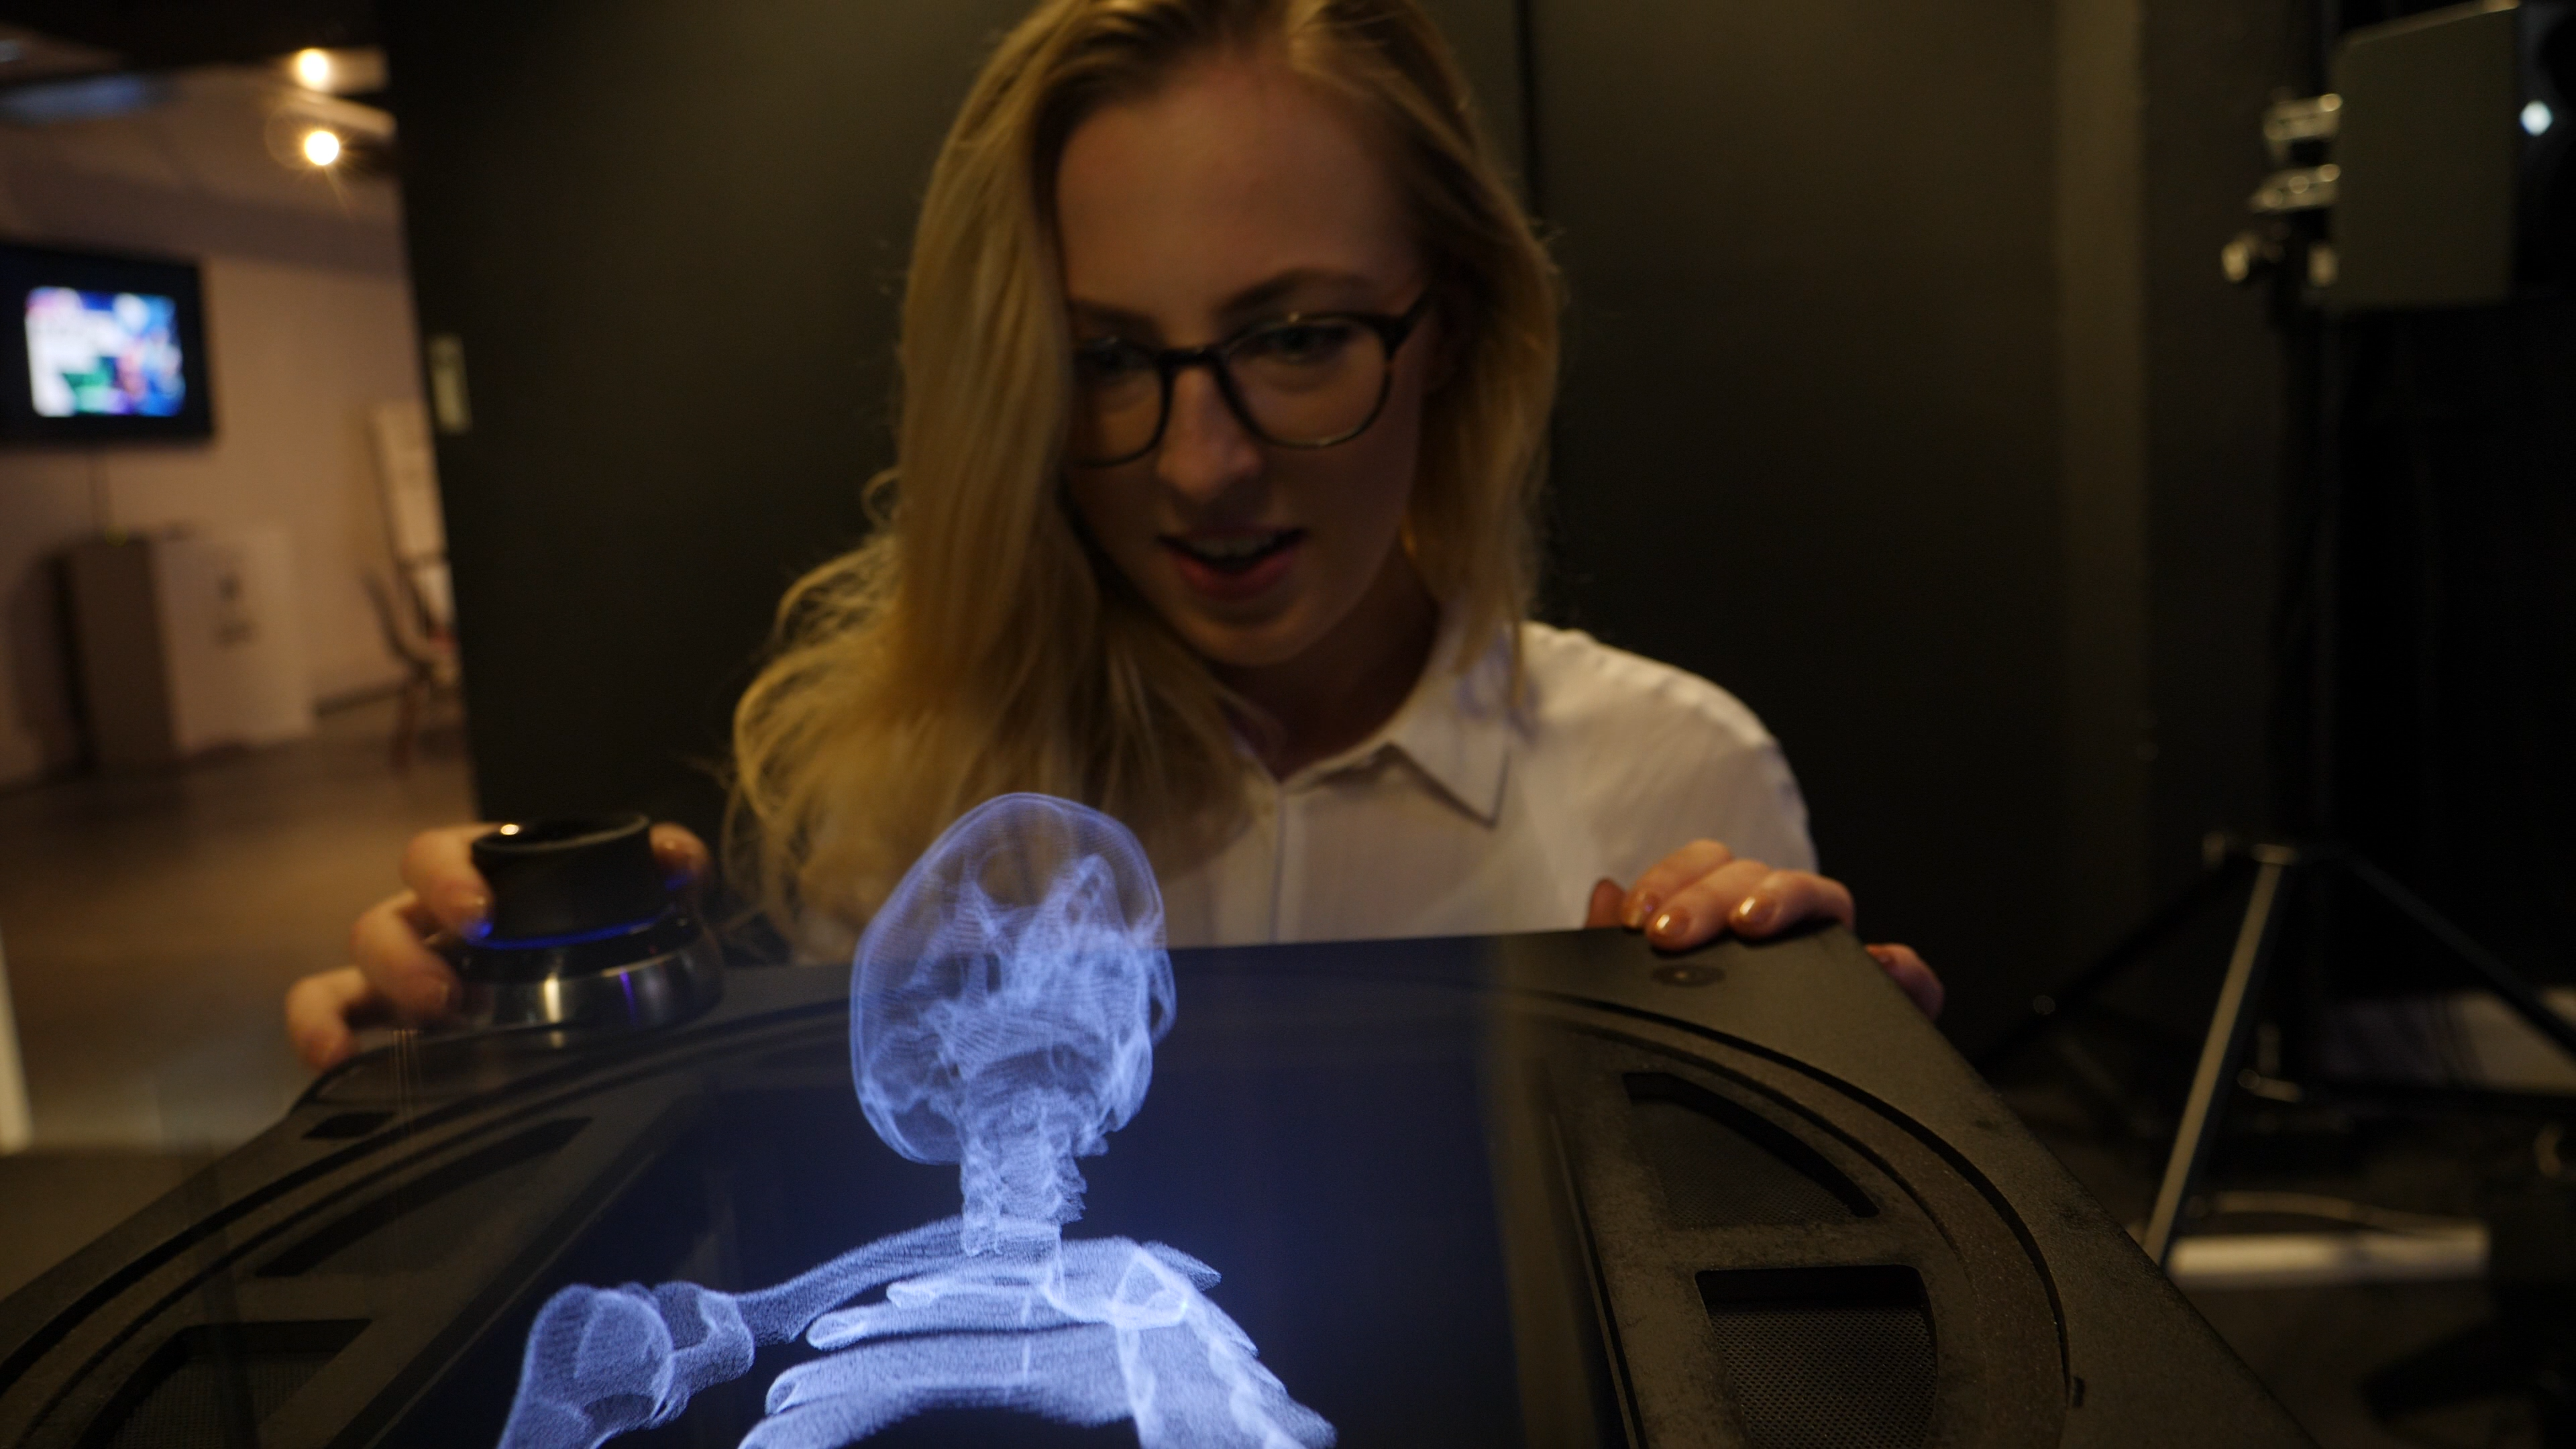
\includegraphics[width=\columnwidth]{Chapter4/Images/stl_bones0.png}
    \caption[An image of a set of bones from a CT scan displayed as an iso-surface on a volumetric display (the Voxon).]{An image of a set of bones from a CT scan displayed as an iso-surface on a volumetric display (the Voxon). This image was provided by Voxon Ltd.}
    \label{fig:VoxonImageOfMedicalData}
\end{figure}

Volumetric displays such as the Voxon~\footnote{\url{https://voxon.co/}} generate a true 3D image by moving a screen rapidly up and down.
This creates a display that appears very similar to real-world 3D objects that can be viewed from almost any angle. 
A short project was undertaken to determine if it was possible to display \gls{ct} or \gls{mri} data using \gls{dvr} on a volumetric display. 
This included trying to visualize small \gls{dicom} files on the device. 
This project quickly failed due to limitations caused by this type of display and the required power. 

The lack of occlusion is a challenge with bringing \gls{dvr} to this technology. This is difficult due to the lack of occlusion possible on these displays, causing issues in determining the depth of certain objects~\cite{Geng2013}.
This is compounded by the fact that these \gls{dvr} objects require a dense grid of \glspl{voxel_g}, requiring a good sense of depth to distinguish the difference between different elements.
The relatively low refresh rate caused by all of these components makes this difficult, and this can be more challenging when projecting more than one color. 
Volumetric displays tend to require high-speed projectors, and many of these only produce a small amount of colors and shades due to their low bit rate~\cite{Nakagawa2023}. 
If it were possible to transfer a form of direct volume rendering to this technology, all this would need to be considered.

This type of display, however, could better be utilized by showing an adaptive version of an iso-surface-like matching cubes as can be seen in \autoref{fig:VoxonImageOfMedicalData}.
The design allowed for an interactive display that could show the most possible detail to the end users.
While \gls{dvr} is not well suited to volumetric devices, iso-surfaces are a viable option. 

% The Looking Glass Demo
\subsection{Autostereoscopic Displays} \label{sec:AutoStereoscopicDipslays}
% Talk stereoscopic displays in general
Auto-stereoscopic displays aim to let users see a 3D image without needing any special eyewear.
This makes auto-stereoscopic displays well-suited to shared experiences. 
This method could allow patients and a doctor to talk and view a \gls{dvr} visualization together, allowing for clearer communication between medical practitioners and patients~\cite{Ni2011, Abildgaard2010}. 

The display used for this project was a Looking Glass~\footnote{\url{https://lookingglassfactory.com/}}, which used a Lenticular-Based Display.
Lenticular Autostereoscopic displays present a series of images or views that are sliced and interlaced. 
As the viewer changes their viewing angle, different images are visible to each eye, creating a 3D effect.

\begin{figure}[tb]
    \centering
    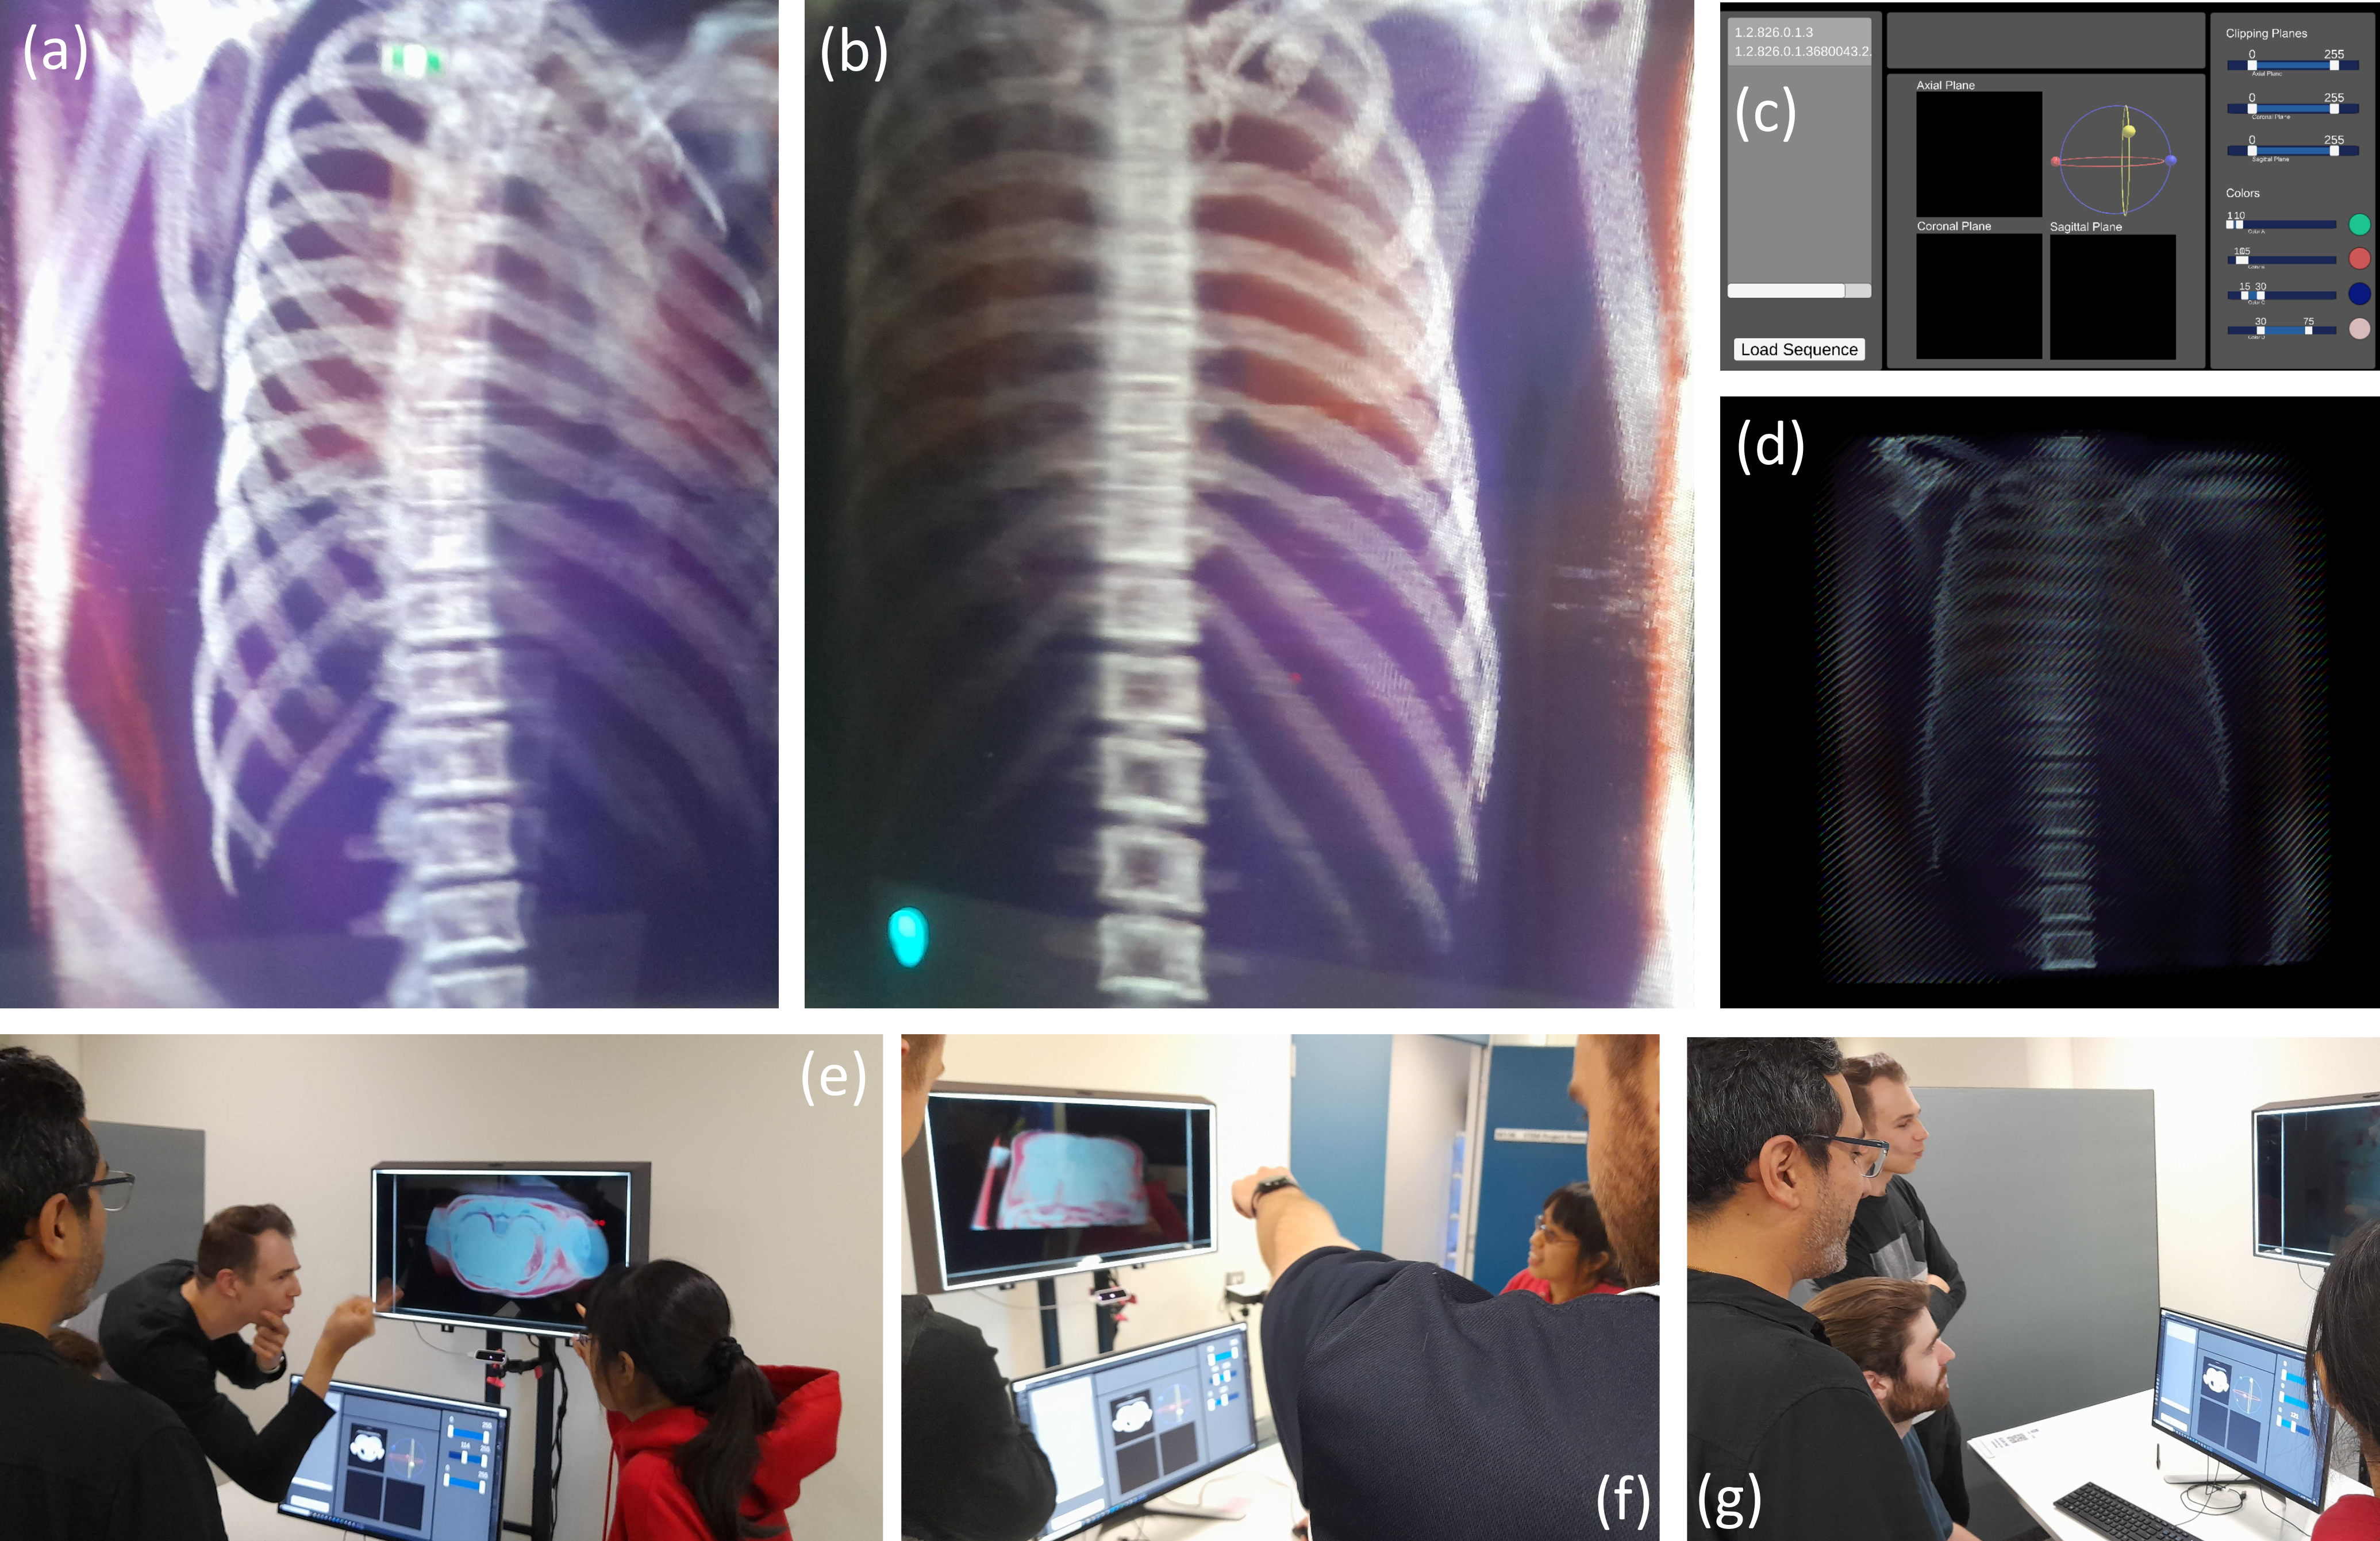
\includegraphics[width=\columnwidth]{Chapter4/Images/AutoStereoscopicDVRForMedince.png}
    \caption[A series of images showing the looking glass prototype utalizing \gls{dvr}.]{A series of images showing the looking glass prototype utalizing \gls{dvr} (a and b) show pictures of the display looking the same volume from two different angles (a) is from the left and b is from the right (c) shows the prototype's interface (d) shows the same image as seen in sections a and b. (e, f, and g) presents a collection of users using the system simultaneously.}
    \label{fig:AutoStereoscopicDVRForMedince}
\end{figure}

This project found that autostereoscopic displays are a good opportunity. They are similar to traditional displays but take advantage of many different views that humans require. 
Autostereoscopic technologies have a limited depth plane. Anything in the foreground or background of these technologies would be blurred out due to the binocular disparities caused by the mismatch between the two displays. 
This allows for \gls{dvr} to benefit from a more natural feeling of depth perception with very little work, as even if all the user can see is the first pane, the difference between the displays each user can see will still create this stereoscopic effect.

One challenge to note that \gls{dvr} has when being used on an Autostereoscopic display is rendering time.
Displays like the Looking Glass may have up to 100 different viewpoints, each of which needs to be rendered in each frame. 
This can make interacting with the volume directly a challenge.
Early testing of the demonstration and user testing of these systems show that frame rates over 20 \gls{fps} are tolerable or unnoticeable, and frame rates above 5 \gls{fps} can be tolerated. % I do not think anyone has done this research

Since this system functioned similarly to a traditional desktop display, caching was utilized to accelerate the frame rate when the \gls{dvr} visualization was static.
This caching allowed the \gls{dvr} to step through 256 times, even at a much higher-than-normal resolution. 
Early ray termination was utilized once the color could no longer be changed or when the ray left the \gls{aabb}. 
However, the step size was decreased to allow for more steps to allow a higher resolution from the device.

The prototype seen in \autoref{fig:AutoStereoscopicDVRForMedince} was designed as a second step to help us understand how Autostereoscopic displays should be built for surgeons and medical practitioners based on a prior investigation with two surgeons who wanted to learn if a 3D visualization could change the method they prepared for dangerous surgeries. 
The original prototype these surgeons interacted with utilized 3D visualization consisting of a stack of 2D planes whose orientation could be viewed from the Axial, Coronal, or Sagittal planes depending on the angle from which the volume was being viewed.
Most of this system's design functionalities have been informed by surgeons themselves.
Including the need for \gls{dvr} to be utilized along with traditional 2D \gls{ct} and \gls{mri} scans. 
They also wanted to restrict the volume they were looking into and control the system either from the 3D perspective for the patient's well-being or from the 2D perspective, which they had more experience with and gave them more precise control. 

As well as utilizing real-time \gls{dvr} for this project, this system required several more attributes. 
This system was required to be able to read any MRI or CT data and render it as a volume while using the same dataset to power other options.
This prototype could load many different volumes at once and enabled quick switching between them.
It utilizes real-time clipping planes and lets users change some of the properties of the transfer process (Opacity, Color, Gradient). 

In this state, it was demonstrated at Aus Medtech 2024, where it was shared with the Australian medical community.
From here, marketing and patient communication cases were suggested for the following product. 
It was also considered a mechanism for remote communication between medical practitioners and patients to discuss their medical scans.
This would help enable communication between hospitals to collaborate on a given patient with little concern. 
More research is required to determine the steps required for its use in diagnosing patients and surgical assistance.

% You could note that interactions with these technologies could be interesting

\subsection{Stereoscopic Head Mounted Displays} \label{sec:StereoScopicHMDsAndDVR}
% Talk about OST AR displays and the limitations. 
%Stereoscopic \glspl{hmd} tend to have a different set of limitations to the previous set of displays mentioned in \autoref{sec:AutoStereoscopicDipslays} and \autoref{sec:VolumetricDisplays}.
Stereoscopic \glspl{hmd} encompass any \gls{ar} or \gls{vr} \gls{hmd}, which places a different screen in each eye and tracks the user's movement.
Allowing the users to be fully immersed in the virtual environment. 
Similar to the autostereoscopic displays in \autoref{sec:AutoStereoscopicDipslays}, the volumes must be rendered at different levels, but there are due to the screen's position, some other tactics are required due to the different methods of interactions possible.

One difference between producing volume rendering on a \gls{hmd} rather than a screen-based device is that you can walk around the volume. 
They allow for better depth perception since they allow for binocular depth cues and motion parallax-based depth cues, which can be triggered even by utilizing the most minor movements. 
Rendering all these changes to the volume caused by these little movements makes using a \gls{dvr} difficult to visualize, causing most people to contain the research into this space into a cube~\cite{Fischer2020}.
Volume rendering is also usually visualized using a plane, but it requires a 3D object when using a Stereoscopic \glspl{hmd}. 

\autoref{fig: Examples of how volume rendering polygons} Illustrates the importance of utilizing the outer polygon shape to match as closely as possible to the outer shape of the polygon case to aid the system's own calculated binocular distortions~\cite{Heinrich2022, Kersten2006, Kersten-Oertel2014}.
Most volumes use a rectangular prism as their base shape due to its grid-like structure and the computational advantages it can assume.
Cubes also utilize the fewest polygons possible, which slightly improves rendering performance. Vertex operations only need to be called 24 for any view, so any eye sees the box.
This effect may not be evident when viewing the volume from a distance, but when close to the visualization, the volume may appear slightly displaced~\cite{Vishton1995}. 
Using a cube to display a volume generally provides acceptable depth on a stereo headset. Some users might experience distortion due to the absence of depth cues that the surrounding environment typically provides. 
Additionally, placing the volume within a more closely fitting mesh to its base shape can enhance near-field interactions, as the amount of white space constrains interactions with the volume or close examination on a conventional mesh. 
The systems in this thesis employ closer-fitting meshes for Volume Rendering.

\begin{figure}[!tbp]
    \centering
    \includegraphics[width=\columnwidth]{Chapter4/Images/AlternativeDVRPerspectives.png}
    \caption[A third person view of Direct Volume Rendering using three different polygonal meshes.]{A third person view of Direct Volume Rendering using three different polygonal meshes. In the green box the outputs from the cameras by looking at each of the different meshes. The straight lines coming from the camera represent the camera frustum.}
    \label{fig: Examples of how volume rendering polygons}
\end{figure}

% % The pros and cons of using cubes for volume rendering
% This effect may not be evident when viewing the volume from a distance, but when close to the visualization, the volume may appear slightly displaced~\cite{Vishton1995}. 
% Conforming the outer shell of the volume has been proposed as a mitigation strategy to address this issue. 
% While using a cube to display a volume generally provides acceptable depth on a stereo headset, some users might experience distortion due to the absence of depth cues that the surrounding environment typically provides. 
% Additionally, placing the volume within a more closely fitting mesh to its base shape can enhance near-field interactions, as the amount of white space constrains interactions with the volume or close examination on a conventional mesh. 
% The systems in this thesis employ closer-fitting meshes for Volume Rendering.

\subsubsection{Challenges Regarding Frame Rate}
Wang et al.~\cite{Wang2023} state that \gls{vr} \glspl{hmd} require a frame rate of 120 fps to avoid simulator sickness and increase the speed of the user interaction.
This is much higher than a traditional display would be expected to run at, making it difficult for \gls{dvr} applications to run on stereoscopic \glspl{hmd}.
%Frame rate is the other issue that needs to be noted.
Having two separate displays that are being shown to users makes the frame rate twice as difficult to manage as it would generally be. The slower frame rate will cause the user to perceive a blurring effect~\cite{Zhao2022}.
Users move quite regularly and require the visualization to be refreshed as much as possible~\cite{Wang2023}.
This is a challenging task on \gls{ost} \gls{ar} \glspl{hmd} as many of the devices are designed to be mobile.
Calculating the position of real-world objects is also a challenge for \gls{ost} \gls{ar} \glspl{hmd}, which requires sensor information to locate real world elements rather than just being able to rely on RGB camera imagery~\cite{Zari2023}.

\subsubsection{Challenges related to Occular See-Through Head Mounted Devices}
\begin{figure}
    \centering
    \includegraphics[width=\textwidth]{Chapter4/Images/ColorsOnDifferentDevices.png}
    \caption[This figure shows images from a computer monitor, an AR overlaid image, and the HoloLens2's display directly, featuring a box with a wireframe version of \gls{X-ray Vision} that can cast a shadow over the unseen area.]{This figure shows images from a computer monitor, an AR overlaid image, and the HoloLens2's display directly, featuring a box with a wireframe version of \gls{X-ray Vision} that can cast a shadow over the unseen area. A set of red, blue, and green lights is directed at this object, showing almost the full-color gambit.}
    \label{fig:ColorsOnDifferentDevices}
\end{figure}


%\gls{OST} displays have the same limitations as the \glspl{hmd} noted in \autoref{sec:StereoScopicHMDsAndDVR}. 
%These tend to come from their use of color. 
Realistic color representations are challenging on different displays, and \gls{ost} \gls{ar} devices further complicate this issue. 
Unfortunately, each device brings its problems, such as what color gambit they can display, the contrast they bring to the real world, how much of the users' real vision is occluded, and the specific configurations of how the virtual and the real worlds are viewed~\cite{Erickson2020, Lee2020, Ashtiani2023}. 
\autoref{fig:ColorsOnDifferentDevices} shows the gradual color change between a computer display and an OST AR display. The OST AR display amplifies the brightness of the colors than intended, whereas the VST AR overlay struggles to choose between the foreground and the background colors. 
The observed changes come from several hardware limitations and user preferences on the mentioned devices.

\autoref{fig:ColorsOnDifferentDevices} highlights a range of colors that \gls{ost} displays ca not properly display.
These relate to colors that are considered dull (colors that utilize a lot of brown or black) as projecting these colors vibrantly is difficult~\cite{Lee2020, Ashtiani2023}.
This makes these colors appear both dull and translucent~\cite{Erickson2020}.
This means that bright and clean colors are really the only viable solutions for these \gls{ost} devices.



\begin{figure}[bt]
    \centering
    \includegraphics[width=\columnwidth]{Chapter4/Images/RealTimeVolumeRenderingExamples.png}
    \caption[This image showcases some examples of what is possible for real-time volume-rendered graphics working on an immersive \gls{mr} \gls{hmd} running at 60 fps on a GeForce RTX 2700 \gls{gpu}.]{
    This image showcases some examples of what is possible for real-time volume-rendered graphics working on an immersive \gls{mr} \gls{hmd} running at 60 fps on a GeForce RTX 2700 \gls{gpu}. a) heptane Gas simulation, b) CT scan of a monkey, c) Visible Human Male, d) CT scan of an orange, e) Upwind information from Hurricane Isabel,  f) Visible Human Female.}
    \label{fig:RealTimeDVR}
\end{figure}

\subsection{Implementation Details}

Applications of \gls{dvr} that were utilized in this dissertation utilized this version of \gls{dvr}, which can be viewed in \autoref{fig:RealTimeDVR}.
This version of \gls{dvr} was designed to be very efficient but also allowed for multiple colors to be represented using different ranges of \gls{hu} and \gls{tesla} values.
These colors utilized a look-up table, which held information relevant to the two different color blending techniques.

Before running this system, each \gls{voxel_g} was split into components either outside of the main body (outside), inside of the main body (inside), or inside the main body but touching the outside (surface) by running a volumetric recursive 12-directional \gls{bfs}. 
The distance between all outside and surface boundaries was then calculated and stored within the volume.
Then, the \gls{hu} or the \gls{tesla} values were pre-allocated with a known min and max attributed to the \gls{dicom} value before the system applied these values.
All values in the volume were then normalized and sent to the shader via a 3D texture.
The color values were used to store the \gls{voxel_g} data, where 1 unit stored the \gls{hu} or the \gls{tesla} values, and another unit stored the relative distance to the nearest surface \gls{voxel_g}.

\begin{figure}
    \centering
    \includegraphics[width=\columnwidth]{Chapter4/Images/TransperentSDFSphereAndRayMarching.png}
    \caption[A diagram of how ray marching works regarding this implementation of SDFs.]{A diagram of how ray marching works regarding this implementation of SDFs. 
    The dotted blue line circles are the ray logic, moving forward until the nearest part of the ray enters the volume. The green dots (Step Positions) represent each step the volume reads to produce the value for a single pixel. While outside of the SDF, sphere marching was utilized whenever outside of the object to reduce the number of steps required. If the ray is close to the object or inside of it, the algorithm becomes ray marching, where we move forward by a specified amount for each interaction.}
    \label{fig:SDFRayTracingDiagram}
\end{figure}

The relative distance to the nearest surface was calculated by normalizing the distance between two of the furthest corners on the volume boundaries and then normalizing all other distances to the same coordinates.
The shader also needed to perform the same calculation to accurately correct this distortion, allowing it to perform the space-skipping procedure shown in \autoref{fig:VoxelBasedSphereMarching}. 
% Talking about how this was implemented in this thesis
By having the relative distance from any space on the volume, a form of empty space skipping that resembled sphere marching (shown in \autoref{fig:SDFRayTracingDiagram}) was also utilized by calculating the distance from the center of a \gls{voxel_g}(\textbf{c}) to the center of a surface \gls{voxel_g}(\textbf{s}) allowing for large gaps to be quickly traversed~\cite{GPU_Gems2}. 
\(distance(\mathbf{c}, \mathbf{s}) = \sqrt{\sum_{i=1}^{n} (c_i - s_i)^2}\)
This requires preprocessing as all of the distances between the \glspl{voxel_g} that are on the surface (\textbf{s}) of the volume will need to be rendered, resulting in the \glspl{voxel_g} acting as an estimate to the next object, as shown in \autoref{fig:VoxelBasedSphereMarching}. 


The same implementation used for the empty space skipping could have also been utilized when traversing through the volume by grouping areas of similar \glspl{voxel_g} to allow for adaptive sampling.
This could have been done by setting a tolerance value and grouping all values that were of a similar \gls{hu} or \gls{tesla} value range, which could have been skipped, and the color value would have been calculated to be identical as if the system did the process the same.  
This was not utilized as it created visual artifacts that made it distinct from regular \gls{dvr}, potentially causing it to hide information~\cite{Morrical2019, GPU_Gems2}.
Lowering the algorithm's tolerance to react to smaller changes could have increased its accuracy, but due to the high variability of the data, it would have slowed down more than it was initially.

Two options for visualizing the colors: either it applied a flat range to a range of \glspl{hu} to isolate different parts of the volume, or it performed Interpolation between the different ranges to better highlight the different parts of the volume. 
The range base would color space within a range of two \glspl{hu}. This allowed the range-based method to ignore certain values within the volume and ignore areas like the bones.
The other option utilized linear interpolation between points. Each point would correlate to its own color, and \glspl{voxel_g} with that color would be the most colored in their given value. Each other color would change gradually and appear closer to its harboring color as the values grew closer to it. 
The linear interpolation volume transformation sets two capstone values less than the minimum, which are black but fully transparent, and any volume above the maximum, which is transparent and clear. 

Getting \gls{dvr} to run on stereoscopic \gls{ost} \gls{ar} devices requires displaying the visualization on two displays and updating them at least 30 times a second. 
Most \gls{ost} \glspl{hmd} are not able to run even the most efficient forms of \gls{dvr} in real time on these displays, as the ones used for this thesis utilized lower-powered mobile hardware~\cite{Jung2022}. 
It is for this reason that this version of \gls{dvr} is designed to run on desktop hardware weathered to an \gls{ost} \gls{ar} \gls{hmd}.

To lower the processing time, the version of \gls{dvr} scattering and other light effects were removed from the algorithm. 
Early ray termination was activated when the color had reached a point where it was not able to change from more steps, the ray leaves the \gls{aabb}, or if the ray required over 126 steps to complete. 
There was no system to cache the rendering, as even slight movements from the headsets would result in a different view of the volume.

\begin{figure}[tb]
    \centering
    \includegraphics[width=\columnwidth]{Chapter4/Images/VoxelBasedSphereMarching.pdf}
    \caption[A 2D example of empty space skipping using a grid-based approach.]{A 2D example of empty space skipping using a grid-based approach. The distance that each moved forward would be equal to the distance to the nearest object. It then moves that much further each time until the distance to the next \gls{voxel_g} is beneath the given threshold, where the ray will then move at the given distance of that threshold.}
    \label{fig:VoxelBasedSphereMarching}
\end{figure}

% Conclude this section
%To get \gls{dvr} working on low-powered \gls{mr} \glspl{hmd}, it is possible its utility would be diminished~\cite{Jung2022}.
The version of \gls{dvr} created for this system is designed to take advantage of techniques that do not decrease the visualization quality in an immersive environment, so elements like space skipping and early ray termination were kept. 
This selection of parameters that controlled the quality of the visualization was tuned to produce an accurate image that can be visualized and modified in real-time on a range of different devices while still providing the best system results. 


\section{X-ray Vision Techniques for Direct Volume Rendering on Ocular See Through Augmented Reality Devices}
% Introduce this section and put forward the concepts that will be carried through
\gls{ost} \gls{ar} allows users to see the real world directly with virtual content overlaid onto it. 
However, in an \gls{ost}, these virtual images can be washed out by light from the real world, so \gls{X-ray Vision} cues are not as strong in an \gls{ost} \gls{ar} device compared to \gls{vst} \gls{ar}~\cite{Martin-Gomez2021}. 
\autoref{Chap:X-ray Implemntion} has shown that four issues need to be considered when creating \gls{X-ray Vision} visualizations for \gls{ost} \gls{ar} \glspl{hmd}:

% Mention again the lessons learned from OST AR Devices
\begin{itemize}
    \item The \gls{X-ray Vision} effect will not be affected by the user's view of the real world but rather by static visualizations. \textit{In \autoref{Chap:X-ray Implemntion} participants found both the camera-based \gls{X-ray Vision} (edge and saliency) effects to be more difficult to use, and they performed worse when using them.}
    \item The \gls{X-ray Vision} effect still needs to occlude the interior objects partially, but not the users' view inside of the object since this allows for additional depth cues like relative size and distance. 
    \textit{The reference objects in \autoref{Chap:X-ray Implemntion} proved to be beneficial to \gls{X-ray Vision} as they help users locate objects nearby in relation to the interior of each object. This is likely to be very important in volumes as surfaces can be difficult to discern. This effect is made more difficult when you consider all the different surfaces that can exist in volume.}
    \item The \gls{X-ray Vision} effect should also not use large objects as it is designed to be used up close to allow near-field interactions. 
    \textit{Participants mentioned in \autoref{app:Chapter3Comments} both Saliency and Random Dot occluded too much of the interior, causing participants to have issues interacting with the visualization when they were up close.}
    \item The effects would need to be reactive to the user and efficient enough to not impair the visualization's quality. 
    \textit{The None condition in \autoref{Chap:X-ray Implemntion} performed well in the subjective results. Participants noted this was due to it not occluding their vision in \autoref{app:Chapter3Comments}. To compensate for this, the \glspl{X-ray Visualization} in this chapter will only be observable within the peripheral vision of the participant.}
\end{itemize}
Considering these, it is also important to focus on what could and could not be done using volumetric rendering.

% Geometrical concerns
%On top of what we already understand about
The volumes know about their internal geometry, but they cannot adjust to the real-world external shell.
If the quality of the visualization is poor, the rays can also step over the object's surface, depending on the angle being viewed.
This will result in the visualizations not utilizing the device's built-in binocular distortion and the rest.

% issues with  transparency 
It is also important to consider transparency's impact on the interplay between \gls{dvr} \glspl{X-ray Visualization}. 
Studies have shown that transparency can be detrimental to the user's depth perception when done poorly, but it can be an effective depth cue when done well~\cite{Ping2020, Ping2020a, Pisanpeeti2017}. 
%To illustrate the effectiveness of the transparent \gls{dvr}, we show how any information configuration can be easily understood using this cue~\cite{Zhan2020}.
Transperent \gls{dvr} allows focus on important data while ensuring the overall information configuration remains easy to understand~\cite{Zhan2020}.
The \glspl{X-ray Visualization} presented in this section all ensure an interplay between transparent and opaque visualizations by making the illustrative effects opaque against a transparent volume.
Using occlusion to represent a clear foreground.

% How noticeable latency is 
Due to the noticeable latency, performing a single rendering pass with no processing stage was only possible~\cite{Guo2022, Matyash2021}. 
This means that a depth buffer could not be calculated in time for these effects, which restricts the visualizations to only understanding what information is related to the current \gls{voxel_g}'s details. 

% GPU concerns
\gls{dvr} is not as well designed for running on a \gls{gpu} as traditional polygonal assets are. 
%We have tried focusing on computational methods.
To enable this, methods that can be calculated in advance and utilize information from the texture memory have been prioritized. The memory is designed to use the RGB values of the texture as normal values when they correspond to edges, while the \gls{hu} or magnetic radiance value is stored as part of the texture information. Distance values are calculated only for the exterior surface, allowing them to be pre-calculated with minimal computational overhead.

% How noticeable
Given all these considerations, illustrative effects would make the most sense as a type of volumetric method because it allows for the appearance of transparency while using occlusive objects~\cite{Lawonn2018}, and it can be applied to volumetric objects~\cite{Pelt2008}.
Medical journals commonly use hatching~\cite{gray1877anatomy} and have commonly been used to translate volumetric data to a 2D interface~\cite{Gerl2006}.
There are also methods of producing these in monoscopic screens. However, if done in real-time, these should be able to provide a similar effect to a \gls{X-ray Visualization}.


% \section{Demo}
% This demonstration introduces a novel platform for Augmented Reality (AR) enabled \gls{X-ray Vision}. AR \gls{X-ray Vision} needs to show the correct depth via visualizing both the surface and the distance inside of the object~\cite{Avery2009}. Firefighters, medical practitioners, and security personnel, among others, have found benefits in using AR-enabled \gls{X-ray Vision} ~\cite{Bajura1992, Phillips2020, Held2019}. However, it is an open research question in the best way to implement AR \gls{X-ray Vision}.

% %This is different from other works, which superimpose content over the physical object creating, making the virtual content appear closer than it would normally~\cite{Blum2012, Avery2009, Bajura1992}. 
% This demo shows how an \gls{X-ray Vision} effect can be created with Direct Volume Rendering (DVR) present. Previous research has used \gls{X-ray Vision} with Video See Through (VST) displays~\cite{Rompapas2014} or used polygonal shells~\cite{Avery2009}, or a Tunneling method~\cite{Avery2009} to illustrate the depth and the physical layout of the virtual internal structures to the user. 
% Our work is novel since this is one of the first demonstrations to use DVR on an OST AR device in the last decade, and it is the only form of \gls{X-ray Vision} that utilizes volumetric data rather than preprocessed polygonal shells.

% Optical See-Through(OST) AR allows users to see the real world directly with virtual content overlaid onto it. However, in an OST, these virtual images can be washed out by light from the real world, so \gls{X-ray Vision} cues are not as strong in an OST AR device compared to VST AR ~\cite{Martin-Gomez2021}. So, our first aim is to show that \gls{X-ray Vision} and illustrative effects can be effective in an OST display. The second aim of this research is to illustrate the role that transparency can play in X-ray visualization. Studies have shown that if transparency is done poorly, it can be detrimental to the user's depth perception, but when done well, it can be an effective depth cue. To illustrate how effective the transparent DVR is, we show how any information configuration can be easily understood using this cue. We present a simple-to-understand volume structure that can be randomly generated to fit within a set of parameters for proof of concept or controlled user studies.

\begin{figure}
    \centering
    \includegraphics[width = \columnwidth]{Chapter4/Images/AmeliorateV2.png}
    \caption[Artistic images of anatomical images displayed as an \gls{X-ray Visualization} by Dr Joshua Luke Ameliorate.]{Artistic images of anatomical images displayed as an \gls{X-ray Visualization} by Dr Joshua Luke Ameliorate. These images are titled: left) Hypnotic; right) Infinite. They can be found at \footnote{\url{https://www.artstation.com/jameliorate}}. Used with permission from Dr. Ameliorate}
    \label{fig:Ameliorate}
\end{figure}

\section{VIRT: Volumetric Illustrative Rendering Techniques} \label{sec:X-ray vision}
% 
Throughout history, art has given depth to 2D surfaces; these works have simulated transparency and manipulated physics.
Inspiring this research to explore visualizations that covered all prior concerns was to utilize illustrative effects.
Throughout art, education, and pop culture, hatching and stippling have been used to discern surface curvature and surface texture while still allowing the viewer to look inside. 
\autoref{fig:Ameliorate} illustrates the added benefit that these techniques allow you to see through the surface of a girl and directly into her anatomy. 

% Talking about the theory of these systems, to begin with
The illustrations seen in \autoref{fig:Ameliorate} present the effect of looking through a solid matter using occlusive and semi-occlusive illustrative techniques by using partial occlusion, just like the visualizations seen in \autoref{Chap:X-ray Implemntion}. 
This shows that illustrative effects utilize the same effects to present the effect of looking through objects as the \glspl{X-ray Visualization} seen in \autoref{Chap:X-ray Implemntion}. 
%Since \glspl{virt} can illustrate the surfaces of objects without utilizing an occlusive barrier similar to the design of the X-ray visualizations seen in \autoref{Chap:X-ray Implemntion}. 
Similar to tessellation and random dots, they remain static in the real world. They can also be designed to allow for a gradient of transparency, occluding less of the area where the user is looking and more of the area where they are not. 
%The more artistic approach to the field also helps to convey more natural shapes rather than flat surfaces. 

Utilizing effects that are traditionally designed to be seen in 2D should also be more suitable for a \gls{dvr} solution like direct volume rendering. 
Given the 3D nature of many \gls{mr} displays, this is not guaranteed, and the experiments in the following chapters will investigate users' preferences for these effects when used as a visualization.

\begin{figure}
    \centering
    \includegraphics[width=\columnwidth]{Chapter5/Images/HandDrawnVirts.png}
    \caption{Examples of hand-drawn illustrations using the illustrative techniques that inspired the various \glspl{virt} as they would be depicted within art.}
    \label{fig:HandDrawnVirts}
\end{figure}


%Explaining this system.
% Throughout the rest of this thesis, three different visualizations to illustrate \gls{X-ray Vision}: (1) a \textit{stippling} visualization that takes inspiration from Ghasemi et al.'s~\cite{Otsuki2017},
% (2) a \textit{cross-hatching} based which took inspiration from the wireframe effect shown in  (3), \textit{halo}. 
% Both of these effects provide a form of partial occlusion and use the geometric properties of the volume, like the surface curvature, the shape's size, and the user's perspective. 
% This gives the end user the perception that the visualization has been connected to the real world.

% These methods would give it 

\subsection{X-ray Vision of Empirical Volumes} \label{sec:XrayVisionCTAndMRI}
We will be showcasing these techniques using visualizations of \gls{mri} and \gls{ct} data. The data is preprocessed to calculate the areas defined using a tetrahedra-defining volume where surface normals would be expected and then calculate for all exterior \glspl{voxel_g} the distance away from the volume they were to allow for sphere marching. 
%A similar implementation to this was previously done by Rocha et al.~\cite{Rocha2011}.
By preprocessing the volume's surface and all of the \glspl{voxel_g} outside of this space, representing the skin, it is possible to determine the ray's relation to the surface. This shows an effect slightly over the top of the parts of the surface that are visible by the final volume. 


% % Talking about cross-hatching work
% The \textit{cross-hatching} visualization uses a grid with infinite depth facing the user. Lines on this grid were drawn along the interests of the grid, with thickness varying based on the curvature of the surface of the volume. The lines become invisible when facing the user so they can easily see into the volume. 

% % Talking about Cross hatching
% The \textit{stippling} visualization also uses a grid; however, this includes a sphere at a random place within its bounds, leading to variation in the size of the depth and a less ordered visualization. These dots transition from opaque to clear in the user's line of sight and the object's curvature to allow the user to view the inside of the object.


% 
% The internal contents of our visualizations are created from a set of randomly generated noisy hierarchical spheres. These are generated in real-time and must ensure that no object may touch another unless it is inside of it completely. These volumes will then be constructed as a small file and sent over a TCP connection to the system that renders the volume within the X-rayable fields.
% This allows users to view many different volumes appearing inside the various physical objects. 

\subsection{Halo} \label{sec: SDf Implmention Halo}

\begin{figure}[t]
    \centering
    \includegraphics[width=\columnwidth]{Chapter4/Images/HaloVis.png}
    \caption[The Halo \gls{virt} applied to the Visible Female data set overlaid over the 3D printed dataset to provide an \gls{X-ray Vision} effect.]{The Halo \gls{virt} applied to the Visible Female data set overlaid over the 3D printed dataset to provide an \gls{X-ray Vision} effect. This image was taken using the HoloLens2.}
    \label{fig:HaloX-rayVision}
\end{figure}

%Note other papers that have used this effect and areas where this implementation deviates from theirs. 
Halos's outlines and feature lines have been used to improve depth perception ~\cite{Bruckner2007, Zheng2013} and highlight areas of interest within volumes~\cite{Diaz2008, Piringer2004, Marriott}. 
On its own, a halo does not provide much depth perception, but when it is paired with a colored display, then it can distinguish what is in front and behind clearer than transparent objects can~\cite{Piringer2004}.
\textit{Halos} have also been shown to illustrate where the surface of an object is by highlighting the areas of high curvature~\cite{Bruckner2007}.
\textit{Halos} are also useful to give the viewer a clear indication of borders, allowing them to see what is in front or behind a given object.
Allowing \textit{Halos} to highlight the objects in the scene~\cite{Bruckner2007, Marriott, Baumeister2015, Joshi2008}.
\textit{Halo} can also use these clear indications of borders to provide a clearer indication of relative size and density, which was found to be a very powerful depth cue in \autoref{Chap:X-ray Implemntion}.

\subsubsection{Implementation}
%Implementation changes for this effect
Traditionally, the \textit{halo} effect has been utilized using two graphics passes~\cite{Bruckner2007}. 
The first is to build a volumetric depth map, and the second is to render the volume where needed. 
On an OST AR display, this is problematic as minor delays in latency are noticeable, so rather than rendering two passes of the volume, this dissertation presents a system that could draw the \textit{halos} without a depth map.

To help prevent this latency, an alternate shader was utilized that recorded two colors for the ray, one that would have the previous \textit{halo} the ray intersected with and one that did not.
This allowed the system to only show the final halo that was passed through. 
A halo would only be drawn when these rays got close to the end and hit the surface at almost a 90\textdegree angle.
This would be saved to the final output color, but if it were to enter the same object again or become a halo for another object, it would revert to the non-halo version of the output color.
For the purpose of visibility, all the \textit{halo's} 
However, it does have one caveat: it is possible for it to show outlines on the outer areas of the foreground with a very high level of curvature, presenting more information about the shape of the object but occluding the volume very slightly. 


%To help prevent this latency, a shader that recorded a \textit{halo} and one that did not was used.
If the ray were to enter the same object it was nearby, the \textit{halo} generated would be discarded; if the ray entered another shape or came into the range of another \textit{halo}, it would be saved. 
\textit{Halos} would be visualized when the dot product of the normal and the ray direction was between -0.1 and 0.1, about 90 degrees away from the user's line of sight. 
This did result in a bug/feature that can be seen in \autoref{fig:HaloX-rayVision}'s \textit{Halo} image where the curvature of the outer surfaces may show outlines in the foreground around areas where there was a high curvature on the surface causing the \textit{Halo's} color to be displayed on sharper contours of the volume facing the user.
    
%Parameters used specifically for this effect.
A \textit{Halo} would be produced when the dot product of the normal and the ray direction was between -0.1 and 0.1, about 90 degrees away from the user's line of sight. 
A white \textit{Halo} would be drawn if the direct distance to the SDF was less than the given \textit{Halo} tolerance.
All these variables were chosen to limit the number of floating point artifacts that could appear while keeping the size of the lines as uniform with the rest of the visualizations as possible. 

\subsection{Stippling} \label{sec: SDf Implmention Stippling}
%Note other papers that have used this effect and areas where this implementation deviates from theirs.
\textit{Stippling} can be utilized to show the features within an image~\cite{Kim2008} and depth by using several small dots and is capable of giving the artist a higher level of control over showing the surface range than depth perception.
\autoref{fig:HandDrawnVirts} shows how \textit{Stippling} can show curvature, surface depth, and different textures by changing the size, frequency, and pattern of the stipples~\cite{Preim2005}.
Using this effect to aid in the perception of 3D data is not common~\cite{Lawonn2018}, but it was chosen due to its similar depth perception properties as Otoski et al.'s~\cite{Otsuki2017} Random Dot \gls{X-ray Vision} effect~\cite{Lum2002, Salah2006}.

Stippling has not been as extensively tested for depth perception as any of the other \glspl{virt}~\cite{Lawonn2018}. It is more often used to demonstrate rougher surfaces to detail intricate details and decrease distortions when viewing iso-surfaces~\cite{Lawonn2018, Maciejewski2008}.
\textit{Stippling} allows the user to be able to see a series of textures that are laid over each other due to the high range of control it gives artists but also gives them the ability to show the roughness of the surfaces it is displayed upon~\cite{Lawonn2018, Maciejewski2008, Lum2002}.

% \textit{Stippling} allows for a transparent effect on the 3D object, creating a clear and simple effect with transparent objects~\cite{Yuan2005}. 
% \textit{Stippling} can also utilize partial occlusion and movement to indicate basic depth cues, allowing viewers to easily determine where objects are in relation to each other~\cite{Kim2008}.

\textit{Stippling} is used in graphics to showcase transparency~\cite{Pastor2004}, it is more frequently used to show details in textures much more precise than can be seen by shading alone~\cite{Martin2017}. 
In these cases, it would normally be referred to as dithering as it is used in a much less random manner~\cite{Ulichney1988}.
The particle occlusion formed by \textit{stippling} then clearly indicates what object is in front of another surface, avoiding screen door effects, unlike what the effect of rendering multiple transparent polygons may have on each other. 
This makes stippling a logical choice for an \gls{X-ray Visualization}.
%However, when given the wrong set of patterns or applications, stippling may be misleading as a depth cue, leading participants to mistake the location of a given object.


\subsubsection{Implementation}
This design of this effect took inspiration from two works by Lu et al.~\cite{Lu20, Lu2002} focused on a \gls{gpu} version of stippling and Ma et al.~\cite{Ma2018}, who developed a pre-calculated version of stippling that could be used for dynamic environments.
We also took inspiration from the work by Kim et al.~\cite{Kim2008}, who utilized different-sized dots to portray curvature and importance within a 2D image.
%Taking some light cues from works that focused on 2D implementations of this work to help provide some guidance for appropriate methods to adjust this method to work appropriately in a real-time immersive environment. 

\begin{figure}[tb]
    \centering
    \includegraphics[width=\columnwidth]{Chapter4/Images/StipplingOnCTData.png}
    \caption[The \textit{Stippling} \gls{virt} applied to the Visible Female data set overlaid over the 3D printed dataset to provide an \gls{X-ray Vision} effect.]{The \textit{Stippling} \gls{virt} applied to the Visible Female data set overlaid over the 3D printed dataset to provide an \gls{X-ray Vision} effect. This image was taken using the HoloLens2.}
    \label{fig:StipplingX-ray}
\end{figure}

%Implementation changes for this effect.
%Parameters used specifically for this effect.
The stipple effect was applied over a grid using a converged distribution (or blue noise)~\cite{Lloyd1982} to give the dots an evenly placed tone that was not too regular~\cite{Martin2017}. 
This was chosen over a feature-guided method as it would have required multiple rendering passes or generating a 3D texture over the volume\cite{Kim2008}. 
The blue noise algorithm based on Heitz's and Neyret's\cite{Heitz2018} was used to determine where a dot would be rendered over the shape's surface because it was efficient and well suited for \gls{gpu} architecture and was more visually uniform than traditional white noise~\cite{Ulichney1988}.
The final \textit{stippling} design can be seen in \autoref{fig:StipplingX-ray}.

Two major factors impacted the design: floating point errors and data legibility. Made it impossible to render as many dots as those created by Lu et al.~\cite{Lu20, Lu2002} and Ma et al.~\cite{Ma2018} due to a large number of floating point errors that seemed to be caused by rapid movements and stereopsis. 
To overcome this drawback, a graphics card with single or double-precision floating-point calculations would be required rather than the half-precision that could be utilized. 
As a result, the approach of "less is more" was adopted when rendering the dots while still keeping to guidelines proposed by Lu et al.~\cite{Lu20, Lu2002}, like having more dots when on parts of the volume's surface with high curvature. 
%Based on feedback from the initial pilot studies of the later studies in this thesis, the size of each dot was based on the radius and type of the object it was associated with. 
%Smaller objects had fewer larger dots, which were more densely clustered together, while the other outer regions utilized a sparse clustering of smaller of dots.
All the dots were housed in a grid whose sizes range between $96^3$ and $48^3$ units~\footnote{Real world sizes could vary depending on the volumes but were approximately $30^3$cm in this diseration}, ensuring that the outside of the grid was clear and easy to view while the inside was opaque with little to no floating point errors. 

%Using larger dots would have prevented users from distinguishing different objects within the volume. We found that various objects would seem to merge into one when we used larger dots, leading to worse-than-expected results from our pilot participants.

% The alternate version of this effect created for immersive headsets required us to place all the dots into a series of 3D grids that would warp their sizes depending on the curvature of the surface they were placed on and the size of the noisy sphere. 
% These sizes range between $96^3$ and $48^3$, ensuring that the outside of the grid was clear and easy to view while the inside was opaque.
% We would then place the dots in a random location within the grid close enough to the center to not hit the sides of the cell.


%We increased the size of our dots by 50\% for each layer, creating bigger dots that take up more space in a larger grid. We started with the smallest, densest grid possible that we could make, which was $96^3$. This allowed users to look through and have a clear indication regarding the outside volume.

% To differentiate the different layers of each type of object, we displayed the container regions showing the dots within a $64^3$ grid, and the regions that needed to be counted were displayed in a $48^3$ grid ~\cite{Lu20}. This ensured that the outside of the grid was clear and easy to view while the inside was opaque.

All of the dots were placed randomly within the grid.
to ensure that the dots did not overlap with other dots
To create the dots, first, a center point was picked where the outer edges of the dot would not hit the edge of the cell.
The dots were scaled based on their opacity, as the ones closest to the user would be made transparent, while the ones that were rendered further away or not facing the user were displayed as more open. 
%The further away the dots were from the user of the ray would determine how opaque they would appear to the user, but would not impact their size as this would cause the dots to appear and disappear as the user moved. 
This technique was also utilized in the next section (\autoref{sec: SDf Implmention Hatching}).% for the \textit{hatching} implementation as it better illustrated the shape of the noisy sphere objects. 
When the surface curvature increases, the amount of stipples that appear will decrease, similar to works by Lu et al.~\cite{Lu20, Lu2002}. 
This allows the dots to better represent shade and intensity over the volume\cite{Martin2017}. 

\subsection{Hatching} \label{sec: SDf Implmention Hatching}
%Note other papers that have used this effect and areas where this implementation deviates from theirs
Computer-generated hatching was originally formed by trying to make volumes or images look like they have an artistically drawn look to them\cite{Praun2001, Salvetti2020}.
In an artistic context, \textit{hatching} is considered a good method of showcasing transparency~\cite{Yuan2005}.
Different objects will utilize different patterns and densities of the hatching~\cite{Pelt2008}.
This allows for a large amount of flexibility and allows for more complex surfaces to be hatched.

\autoref{fig:HandDrawnVirts} shows how \textit{Hatching} is similar in utility to stippling; it can show differences between curvature position and lighting~\cite{Preim2005, Philbrick2019}.
It can be used to great effect to showcase curvature within using 2D mediums like books~\cite{gray1877anatomy} and desktop applications~\cite{Preim2005, Philbrick2019, Praun2001}, but there are very few examples of hatching being utilized in \gls{ar}. 
Current examples only show it being used as a medium to help create a painterly atmosphere within mobile \gls{ar}~\cite{Chen2011, Chen2012}.

In an artistic context, \textit{hatching} is considered a suitable method of showcasing transparency, which makes it well suited as an \gls{X-ray Vision} effect~\cite{Yuan2005}.
This is achieved by having the hatching of different objects in the hierarchy display a different width, line angle, and density of the hatching~\cite{Pelt2008, Frech1960}.
%This allows for a large amount of flexibility and allows for more complex surfaces to be hatched.

\subsubsection{Implementation}
Rather than try to make an artistically pleasing hatching algorithm, the implementation of \textit{hatching} in this dissertation aims to create a version of \textit{hatching} that is both simple to implement and understand and functional within MR environments for volumetric datasets.
%Implementation changes for this effect.
This method took advantage of \gls{dvr} and rendered a similar implementation of \textit{hatching} to work by Interrante et al.\cite{Interrante1997}. 
To do this, a grid of rectangular prims as SDF and rendered the area that would not be where the visualization could be presented, each with a deformed cube in the center to apply the hatching effect, creating the line effect seen in \autoref{fig:HatchingOnCTData}.
%to give the cubes a pointed edge; they were warped to grow larger when they collided with a surface with higher curvature. 

The \textit{hatching} effect was generated by creating a grid where every cell was 1.2\% of the size of the volume and had a box at the center of that which was 2.4\% of the volume. 
%These values were then times by the $1 + (\mbox{radius of the nearest object } \times 2)$ leading the larger object to have a cell size closer to 2.4\%.
%This resulted in values
This visualization will be shaded lighter when facing the user's direction. 
This is done by altering the transparency by the angle between the surface visualization and the user.
This was done by tracking the dot product, which was more transparent when the dot product grew lower.
This caused the \textit{hatching} effect to disappear when it was not at the point it was closest to the user.
Both of these parameters decrease when representing smaller objects than the object it was representing, causing the hatching effect to appear as a denser grid. 
After the dot product was greater than $0.25$ of the dot product, the hatching effect would incur a tapering effect.
%If the above was triggered when the ray entered a given tolerance where the dot product of the surface was normal and the participant's viewpoint was less than zero.

\begin{figure}[tb]
    \centering
    \includegraphics[width=\columnwidth]{Chapter4/Images/HatchingOnCTData.png}
    \caption[The \textit{Hatching} \gls{virt} applied to the Visible Female data set overlaid over the 3D printed dataset to provide an \gls{X-ray Vision} effect.]{The \textit{Hatching} \gls{virt} applied to the Visible Female data set overlaid over the 3D printed dataset to provide an \gls{X-ray Vision} effect. This image was taken using the HoloLens2.}
    \label{fig:HatchingOnCTData}
\end{figure}

How to orientate the hatching quickly became an issue. 
Generally, hatching is designed to create a static image, so the lighting and shading would have been seen in a static place, with the light source pre-calculated before each image. 
%This would have made the volumes have a gradient of the effect, making parts of them almost impossible to see through and other areas of the hatching invisible. 
Instead, this version of \textit{hatching} treated the user's viewpoint as if it were a light source and made the effect from their point of view.
This made the visualization react to the users' behaviours and allowed them to have their view partially obscured while allowing them to look inside the volume.

%Parameters used specifically for this effect
Several aspects were considered to maintain the aesthetic elements required for \textit{hatching} when transitioning from a 2D to a 3D volume.
The \textit{hatching} effect utilized an SDF of a deformable square grid with infinite depth on the z-axis.
This grid was deformed based on the relationship between volume and the viewer and to have a larger, more opaque line, the further away from the user the normal was facing from the viewer. 
%Smaller objects in the volume would have a denser hash than the larger ones from the larger ones.
%Making it possible to perform the same algorithm to perform the previously mentioned prior in \autoref{sec:X-ray vision}.
%This is treated in the same way as the other volumes, which use a similar technique to showcase the X-ray vision effect. % Fix this Tom

\section{Conclusion}
To create \glspl{X-ray Visualization} for \gls{ost} \gls{ar}, an efficient method for rendering volumes directly to the screen using \gls{dvr} was developed. 
This method was successfully demonstrated on autostereoscopic displays and provided additional rendering time to generate three sketch-based \glspl{X-ray Vision} effects, collectively referred to as \gls{virt}. 
By leveraging sketch-based visualizations, observations were made that allow for the configuration of these conditions for \gls{ost} \gls{ar} devices.
Moving forward, this dissertation will further explore the utility of these \glspl{X-ray Visualization}.

The contributions of this chapter were:
\begin{itemize}
    \item An algorithm displaying how to run \gls{dvr} on a stereoscopic display with minimal distortions and low graphics requirements.
    \item A system designed using a stereoscopic display was to render \glspl{dicom} using \gls{dvr} while providing a reactive user interface, which allowed users to modify the volumes as they required.   
    \item Three new \glspl{X-ray Visualization}, the \glspl{virt}, have been created to allow for \gls{X-ray Vision} on volumes rendered in \gls{ost} \gls{ar} devices which adapt to user behaviours rather than using solely occlusion.
\end{itemize}
%They have designed them with medical needs in mind that can be applied to an extensive range of volumetric and spatial data.



%
%
%
%
%
\chapter{Random Volume Generator: Generating Irregular Hierarchical Objects for Controlled User Studies} \label{sec:VolumetricDataGeneration}

Finding volumetric data that can be utilized reliably for quantitative experiments is challenging.
Methods to obtain volume data are limited. Two methods of creating volume data can occur by using natural means either:
Patient data or artificial data. 
Patient data is generally collected from a spread of patients with similar symptoms\cite{Cocosco1997BrainWebOI} or collected data from relatively healthy patients~\cite{Ackerman1998}. 
The other method of producing volumetric data is to collect artificial data is collected by utilizing geometrical data to represent various natural phenomenon~\cite{neghip,dns,jicf_q}.
These tend to take the form of calculating known an empirically assessed theoretical physical concept, which in turn can be computationally expensive to produce and to manipulate. 


Controlled studies are challenging to perform with data that is limited in these settings because they rely on having hundreds to thousands sets of similar data based on a given condition.
The data needed to be plentiful enough that conditions could be replicated with different data sets over various conditions and conform to the properties of \gls{mri} and \gls{ct} scans while remaining intuitive enough for untrained users to be able to interoperate it.
This section details the methods focused on creating extensible and flexible volumetric data that participants can understand intuitively, regardless of their prior training. 

% Talk about the different types of data that can be read into the systems
Volumetric data is commonly used to interpret the structure of an object, like the human body, underground structures, or weather data.
Typically, the information utilized when requiring direct volume rendering is sourced from the real world using either \gls{ct}, \gls{mri}, or some form of radar technology.
These methods of obtaining volumetric data can be limited and challenging to produce in large quantities. Access to the machines and equipment capable of producing this data is limited, and the skills required make it difficult to automate. 
Most medical data needs to be anonymized, and the patient authorizes the use of it so it can be used for research.
Furthermore, very little volumetric data is explicitly designed for more controlled or quantized studies. 

The Open Scientific Visualization Database~\footnote{\url{https://klacansky.com/open-scivis-datasets}} has a wide selection of datasets available for science, but they are very different and can result in unexpected differences between the different visualizations when evaluated using a controlled study~\cite{Grosset2013}. 
Current solutions for generating artificial data require precise inputs, are challenging to manage, and are computationally expensive~\cite{Bossek2018, Haghighi2017, Meyer_and_Nagler_and_Hogan_2021, Patki2016}.
This section details a method of making simple-to-understand simulated volumetric data, a method to validate that the data is comprehendible, and a modular system allowing for flexible options to evaluate volumetric structures. 

Real-world volumetric data is challenging to share amongst other researchers due to its large file size and privacy concerns~\cite{Fabian2015}.
Medical data privacy is paramount, and there may be restrictions on what datasets can be distributed through research~\cite{Gillmann2021, Nature2023}.  
The size of the compressed data can easily be larger than one gigabyte for a given volume. 
Making sharing datasets difficult~\cite{Fabian2015}. 
%On top of this, high-resolution volumetric datasets file sizes can be greater than one GB in size for each image. 
This size becomes an issue for data sharing in the long term since storing large data sets will likely cost either the publisher or the researchers~\cite{Nature2023}, leading to many problems with long-term data availability. 

Current alternatives for creating controlled studies using volumetric rendering include adding extra information to the limited volumes via adding artificial data. 
These settings do well in recreating scenarios relating to the introduction of medical instruments to a volume and determining the reliability of these visualizations, but the interactions between other objects become more complex.
Another option can be seen by viewing research that utilized synthetically created data~\cite{Englund2016, Englund2018, Kersten2006}.

%that generates a series of random planes of data to view via a 2D display.
%Bifocal displays utilizing volumes within a cube can present noticeable optical artifacts, causing some users to have imprecise depth perception when using immersive displays. 

Synthetically created data has a couple of advantages. First, it allows you to modify and control the data you are using in a given study, allowing for more quantitative data to answer more specific questions. 
Allowing for more replicable and focused studies to be possible. 
Englund et al.~\cite{Englund2016, Englund2018} experiments generated data designed especially for the purposes of testing their research and rendered as static images of volumes for a range of two alternative forced-choice tasks. 
Kersten et al.~\cite{Kersten2006} utilized a fog-like volume made from Perlin noise within a cylindrical object and rotated it to see if users could tell the direction in which it was rotating.  

Creating synthetic data is a common tactic in many other fields as data of any type are hard to come by, and systems need to be tested using flexible mechanics and a wide range of parameters~\cite{Meyer_and_Nagler_and_Hogan_2021}.
These can range from systems designed to create structured databases~\cite{Meyer_and_Nagler_and_Hogan_2021}, networking data~\cite{Bossek2018, Haghighi2017}, or even modifying the original data for testing or publishing purposes~\cite{Patki2016}.

%\textit{find papers that have tried to solve areas in this area\\}
%Deep learning has also been heavily utilized to create various artificial volumes
There have been several attempts at using the tools \glspl{gan}~\cite{Goodfellow2020} and stable diffusion~\cite{Dhariwal2021} to create real examples of medical data~\cite{Pinaya2022, Ren2021, Togo2019, Nguyen2023}. 
These datasets provide use cases for training staff without the need to provide scans of real people, which can benefit tasks such as publishing and sharing medical data with a broader audience~\cite{Togo2019}, training radiologists~\cite{Nguyen2023}, and research~\cite{Nguyen2023, Ren2021}. 
These models utilize a large collection of existing data and aim to create a new data set, which tends to be indistinguishable from the real data~\cite{Togo2019, Ren2021}.
However, controlling the specific qualities in a manner that would be required for a study is not practical yet, and adjustments to this data for quantitative evaluations are not possible yet.

To solve these issues, the Random Volume Generator was created.
Taking into consideration the above parameters, I built a system to generate volumetric data that can be generated for studies in a unique but controllable mannor. 
This software is designed to act as a tool that can be used to generate a unique volume for each interaction of your study that can be customised to fit any type of research that you need to run. 
By utilizing \glspl{sdf} set in a hierarchy of customizable options.
Keeping the system modular enabled it to swap parts in and out, making it work for any study looking to evaluate volumetric graphics.

\section{Noisy Hierarchical Spheres} \label{sec:SystemOverview}
% \begin{figure}
%     \centering
%     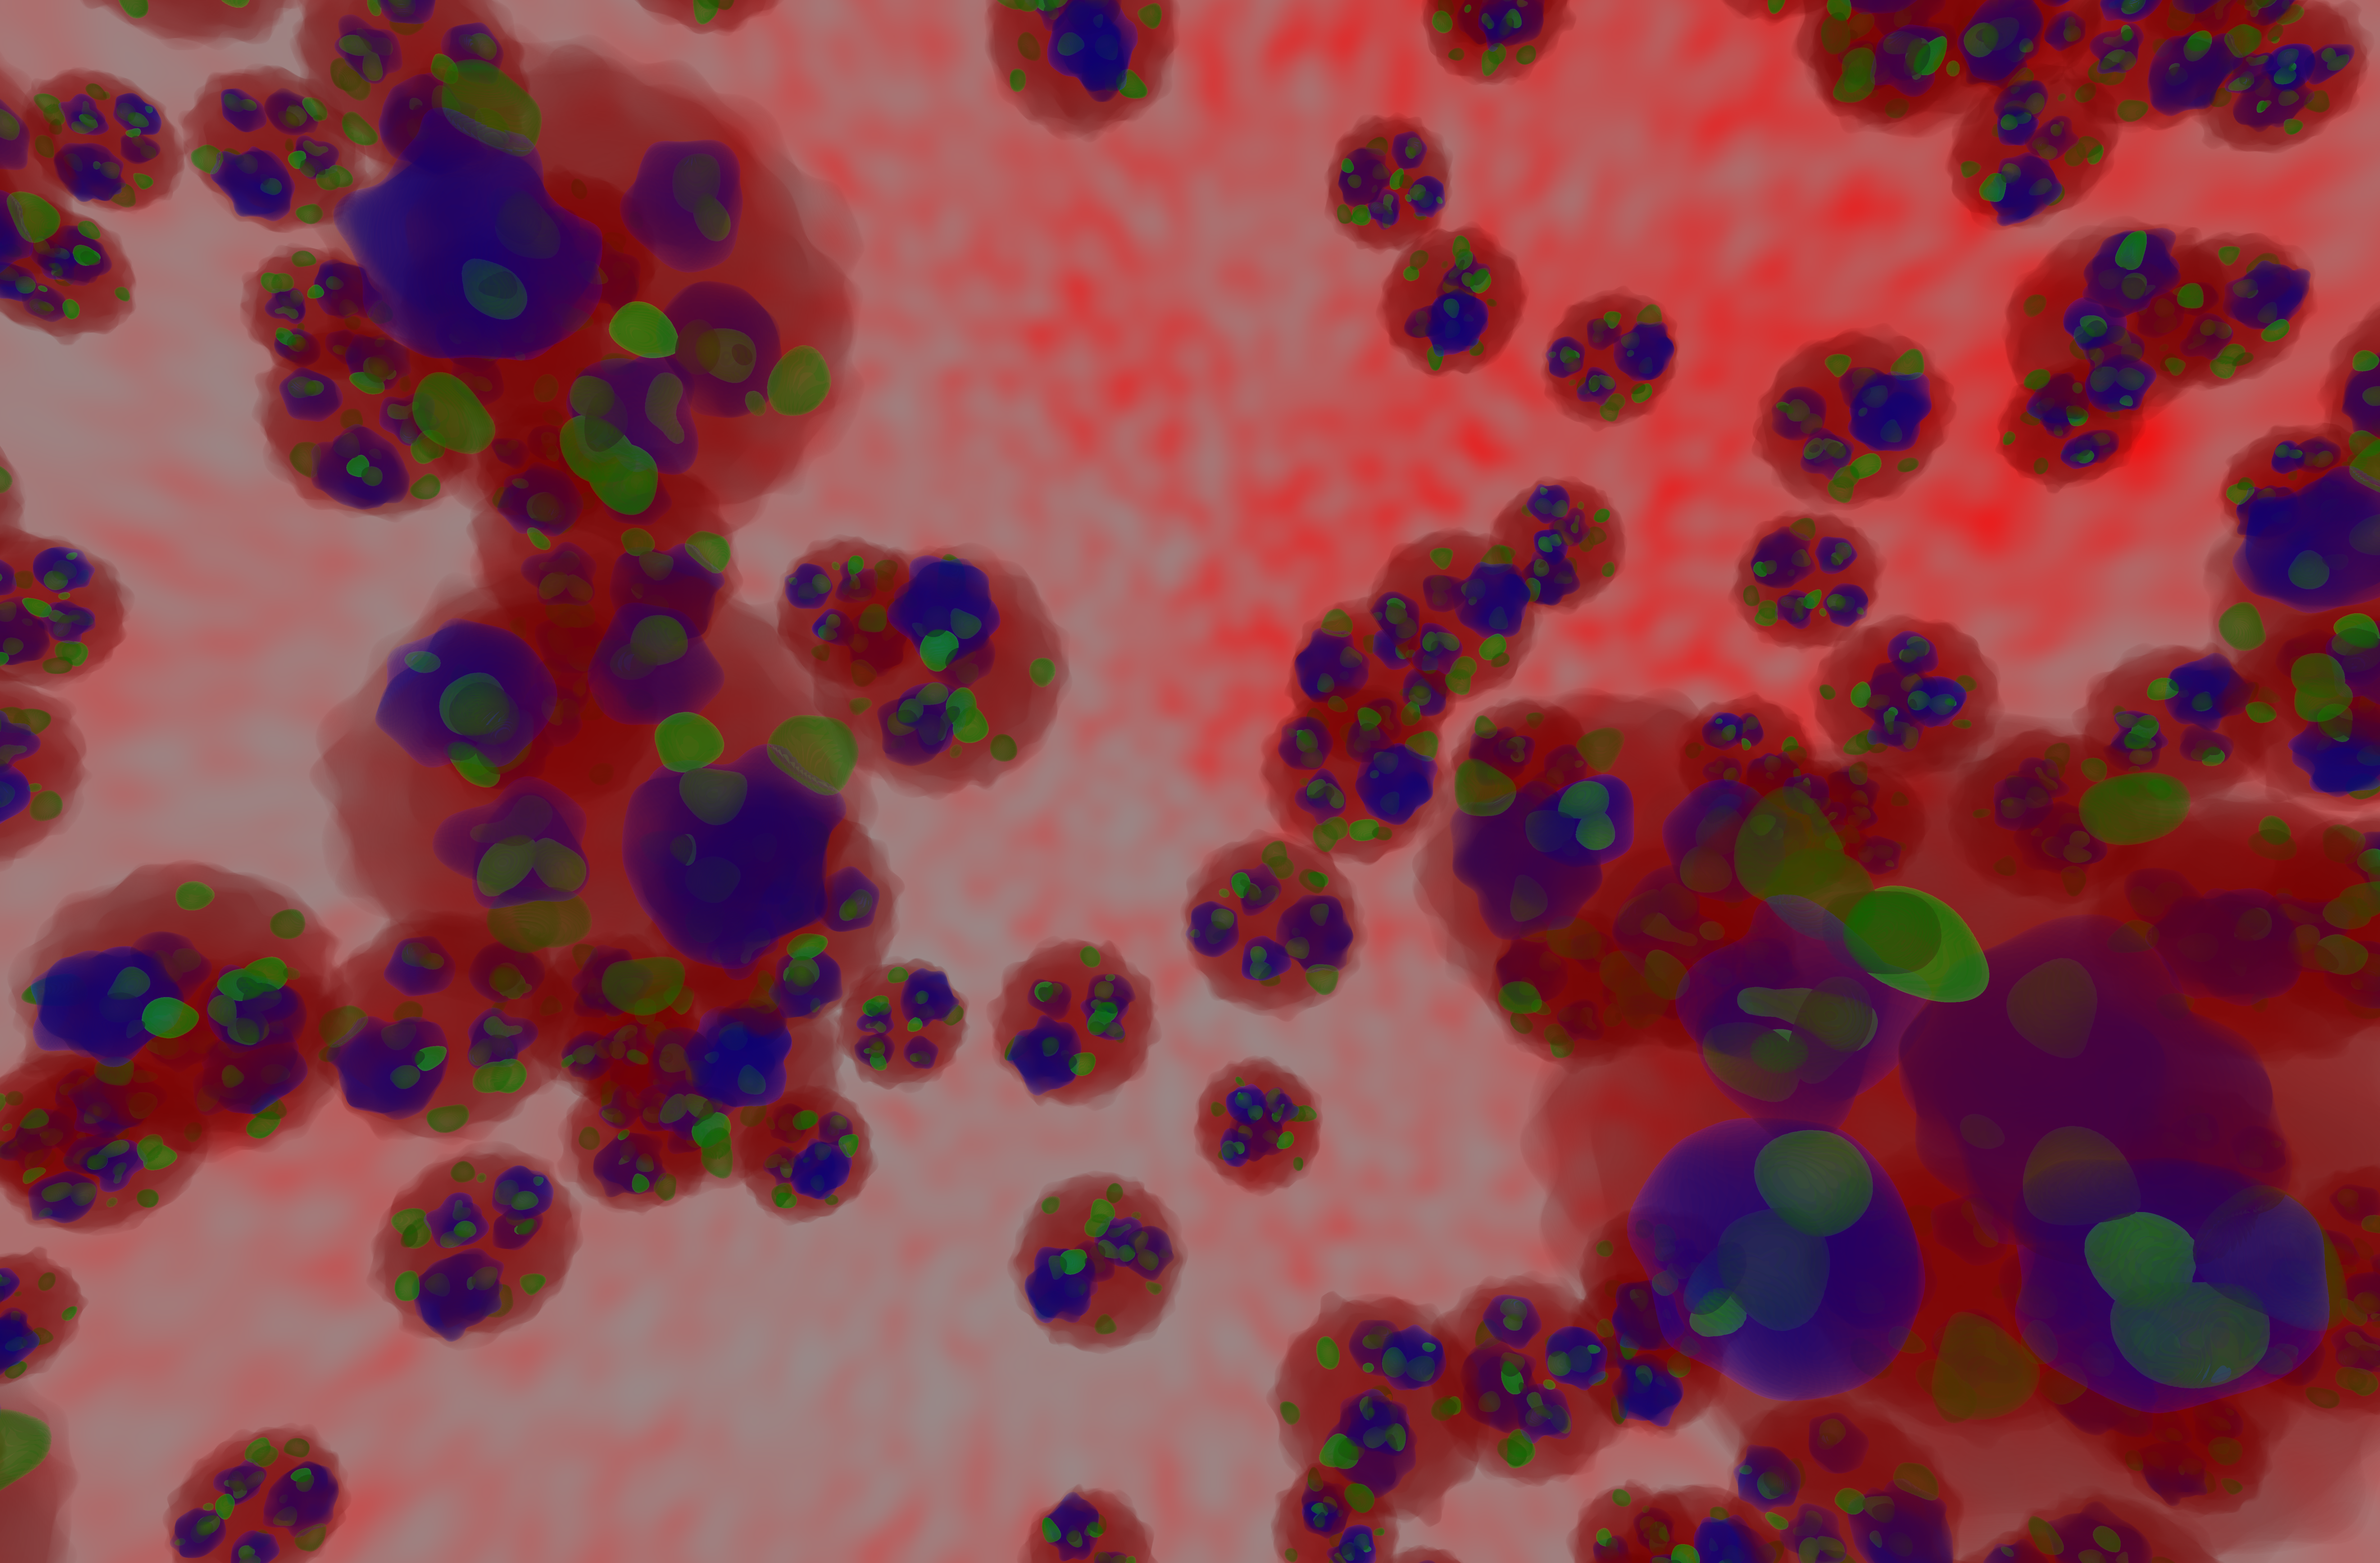
\includegraphics{Chapter4/Images/ImageForResearch.png}
%     \caption{A large amount of the random objects that can be produced from this image are placed in shown all rendering together.}
%     \label{fig:enter-label}
% \end{figure}

% Explaining how the Perlin noise could work
To make these volumes as much like MRI and CT scans as possible, Perlin noise~\cite {Perlin1989} was used to deform a sphere object created via a spherical \gls{sdf} (A noisy sphere) set up in a hierarchical fashion.
Perlin noise~\cite{Perlin1989} is a close match for the noise found in medical data, and it has been utilized to simulate and create artifacts in read medical data for research purposes~\cite{Tomic2023, Lawson2024}.
This results in volumes that appear like the ones in \autoref{fig:noisySpheres}. 
Since they are \gls{sdf}, it is possible to accurately determine the angle of normals in the volume, allowing visualization-based experiments like \gls{X-ray Vision} studies (as seen in \autoref{fig:3DPrintedVersionOfTheSystem}).


We also considered the previous studies that have generated artificial volumes.
Englund et al.'s~\cite{Englund2016, Englund2018} 2D static images would not be translated well to a stereoscopic display as they can not respond to motion parallax.
Kersten et al.'s~\cite{Kersten2006} Perlin noise fog showed promise when using stereoscopic display. 
Perlin noise was adopted to generate synthetic volumes, mimicking the noisy characteristics of volume-rendered objects in applications such as MRI and CT scans.
This approach is advantageous since it can be rendered effectively on a variety of surfaces in real time.
%to some degree was instead chosen as it can be rendered in real-time, and they show that it is not limited to being rendered on planes or cubes.
Volume data tends to be inherently noisy and messy, making it more challenging to interpret, so Perlin noise-based objects make logical sense~\cite{Gillmann2021, Zehner2021}.
The ability to create a solid surface that could represent different materials or densities would be beneficial when trying to create iso-surfaces, and the ability to have identifiable pieces components is common in MRI and CT scans.

%And share qualities that require complex data analytical skills to interpret and tend to require researchers with a multidiscipline skill set. 
\section{Random Volume Generator's System Design}
%NEED INTRO HERE
The Random Volume Generator took on a complex but modular design system in \autoref{app:RandomGerneratingVolumesClassDiagram}. 
Which is designed to produce an array of volumes that can conform to a set of conditions.
This results in the output, which can be seen in \autoref{fig:noisySpheres}, whose shape is a "noisy sphere."~\cite{Perlin1989}.
% Things that happen before creating each volume

Noisy spheres, which are based on a sphere with random distortions, allow for an almost infinite variety of shapes. 
As such, each shape is irregular in nature, and a pseudo-random generation process determines the specific shape and appearance.
All while forcing the dataset to conform to a preconfigured set of requirements. 


% What does this system bring that the other systems didn't
%When designing these volumes, we needed to consider methods like Englund et al.'s~\cite{Englund2016, Englund2018} static images that do not work well on an immersive stereoscopic device. 
The Random Volume Generator is primarily aimed at researchers conducting human-computer interaction research investigating the traits and impacts of different displays and rendering styles~\cite{Rheingans2001, Svakhine2009}.
The volumes generated by the Random Volume Generator need to have generic qualities that other forms of volumes would typically have. 
This might include rounded edges, lumps and bumps around the edges, and a hierarchical set of objects.
We chose to base these volumes on a similar design to MRI and CT scans, but they also share qualities with electron microscopy visualizations~\cite{Nguyen2022}
and with minor modifications, they can be conformed to molecular systems~\cite{Goodsell1989}, meteorological data~\cite{HibbardL.1986, Lin2021}, as well as ground penetrating radar (GPR) data~\cite{Zehner2021}.
All these imaging techniques communicate information via geometrical methods, require a high degree of precision to generate, and are subjective to noise or inaccurate data.

% Make a new Image for this
\begin{figure}[tb]
    \centering
    \includegraphics[width=\columnwidth]{Chapter4/Images/RandomlyGeneratedVolumes.png}
    \caption[The types of volumes the Random Volume Generation System system can produce.]{The types of volumes the Random Volume Generation System system can produce. There are noisy spheres on the bottom and right-hand sides using various illustrative effects (Outlines, Stippling, and Hatching).}
    \label{fig:noisySpheres}
\end{figure}


% the basic algorithm of the system
In each iteration of the generation process (shown in \autoref{fig:ActivityDiagramForGeneratingRandomSDF}), a top-level volume is created and added to the scene. Children within the volume are created recursively. The size and appearance of each volume are determined based on the probability distributions given as input to the generation process, whereby the size of the child volumes is constrained by their parent volume (if any). The number of children in the volume is drawn from a probability distribution for each volume.
In addition, global constraints govern the overall number of objects of each type at each level to ensure that the synthesized scene satisfies the desired properties.

The dimensions and placement of objects are determined at random such that each volume is wholly contained in its enclosing parent volume, and no objects are allowed to touch each other. These placement constraints are verified by a \gls{voxel_g}-based algorithm that examines possible intersections between volumes. The system provides a naive algorithm and a more efficient octree-based implementation. In case an object is found to violate the constraints, the object is moved to repair the situation.

\subsection{System Design}
%This system was designed to be modular.
The Random Volume Generator was designed to be modular by utilizing many system design patterns, interfaces to allow for interchangeable classes, and the use of functors to allow for customizable behaviours.
The system can be split into different parts, enabling adaptation to different requirements.
The different parts of the Random Volume Generator are classified as the Generator builder (used to construct the final structure of the Generation system), the Random Volume Builder and Validation (used to create and validate the success of the valid creation of a valid volume), and the system Outputs (used to tailor the outputs to the various studies that these volumes could be used for).
%All of these systems could then be further modified and changed to allow for more minor changes. 
Class diagrams showcasing the Random Volume Generator's structure can be found in the \Cref{app:RandomGerneratingVolumesClassDiagram}.

Four different types of noisy spheres can be made for the base version: outer, composite, leaf and some multipurpose spheres can also be added. 
%This system uses a series of visualizations that utilize a set of spheres that are deformed by Perlin noise~\cite{Perlin1989} and displays different hierarchies as different objects using different colors. 
To improve optical focus, using the method described in \autoref{Chap:VolumetricX-rayVision} where volumes were housed in meshes that represented the exterior of their shape to some degree, these objects are housed within a spherical mesh.
%\autoref{fig:DifferentVolumeRenderingViews} shows this allows for better bifocal viewing by allowing the mesh to align with the volume. 
Improving the distortion from the bi-optical, allowing for better depth perception~\cite{Kersten2006}.

%
%It needs to perform, and 2 to provide the correct verification for the stage of the volume.
The Unity game engine~\footnote{\url{https://unity.com/releases/2022-lts}} limits the amount of threads available to the Random Volume Generator is required to work within a single thread framework and utilizes active interfaces in tandem with a stateful logic system. 
Systems that handle the system's logic are functors, allowing a system to progress statefully.
Their behaviour is again modular, with the system's logic separated from their unique tasks. 
Allowing for a system capable of doing much more than its base functionality. 
Two simple examples of the methods are recursively placing an SDF within its parents so it takes as much space as possible.
The other can produce several meshes for 3D printing(seen in \autoref{fig:MeshVersionOfTheSystems}) while also providing their corresponding noise key, allowing for comparisons with real-world objects.

\subsection{Voxel-Based Verification of Volume Requirements}

The Random Volume Generator utilized a modular verification system to ensure the volume elements remained distinct to prevent any ambiguity between the objects.
% A brief overview of the volume rendering system
By looking at each \gls{voxel_g} and determining if they are sitting wholly inside each other and not slipping outside their parent object or touching any other object that is not a parent of theirs. 
%These rules can be easily exchanged for any class that inherits the Irules interface. 
The rules are checked via a C\# based system that emulates the same properties of Unity's high-level shader language (HLSL). 
It is designed to be extensible to allow for any SDF and potentially a different type of shader altogether. 

% Explaining how the root objects work
The verification methods for the root (outer) objects check that the volume fits within the mesh within which it is rendering while remaining as large as possible.
This mesh can either be a cube mesh or a spherical mesh.
If any \gls{sdf} is outside of the mesh, the object is discarded, and a completely new object is generated. 
The sphere mesh utilized a Fibonacci sphere algorithm to determine if the large outer sphere was within bounds~\cite{Gonzalez2010} whereas others, like the cube meshes, tested if the mesh was inside of \gls{aabb}.
In both conditions, if any point from any of these checks were found to have any SDFs within a range of them, it would then shrink the volume and perform the check again. 

% The different types of verification
The verification used for the leaf and composite objects can use two different verification methods. 
Either a brute force or progressive oct-tree searching method.
This can either happen linearly or in parallel for each \gls{voxel_g}.
The other method utilizes a partial linear oct-tree starting from one predefined depth in the oct-tree from one depth to another deeper one.
Studies in this thesis utilized an oct tree starting with one layer beneath its root $1/8^3$ to a leaf node that was of a \gls{voxel_g} with the comparable size of $1/512^3$.
This will perform a trimmed depth-first search. 
This search will determine if a group of \glspl{voxel_g} conform to SDF coordinates to ensure that all child nodes are completely within the parent's bounds. 
These brute force and progressive oct-tree can be combined for both high perception and speed.

\begin{figure}[bt]
    \centering
    \includegraphics[width=\columnwidth]{Chapter4/Images/UML Activity Diagrams (Community).pdf}
    \caption{An activity diagram showing the transition between the various states of the Random Volume Generation System}
    \label{fig:ActivityDiagramForGeneratingRandomSDF}
\end{figure}

\subsubsection{Random Volume Generation System Outputs}
\begin{figure}[bt]
    \centering
    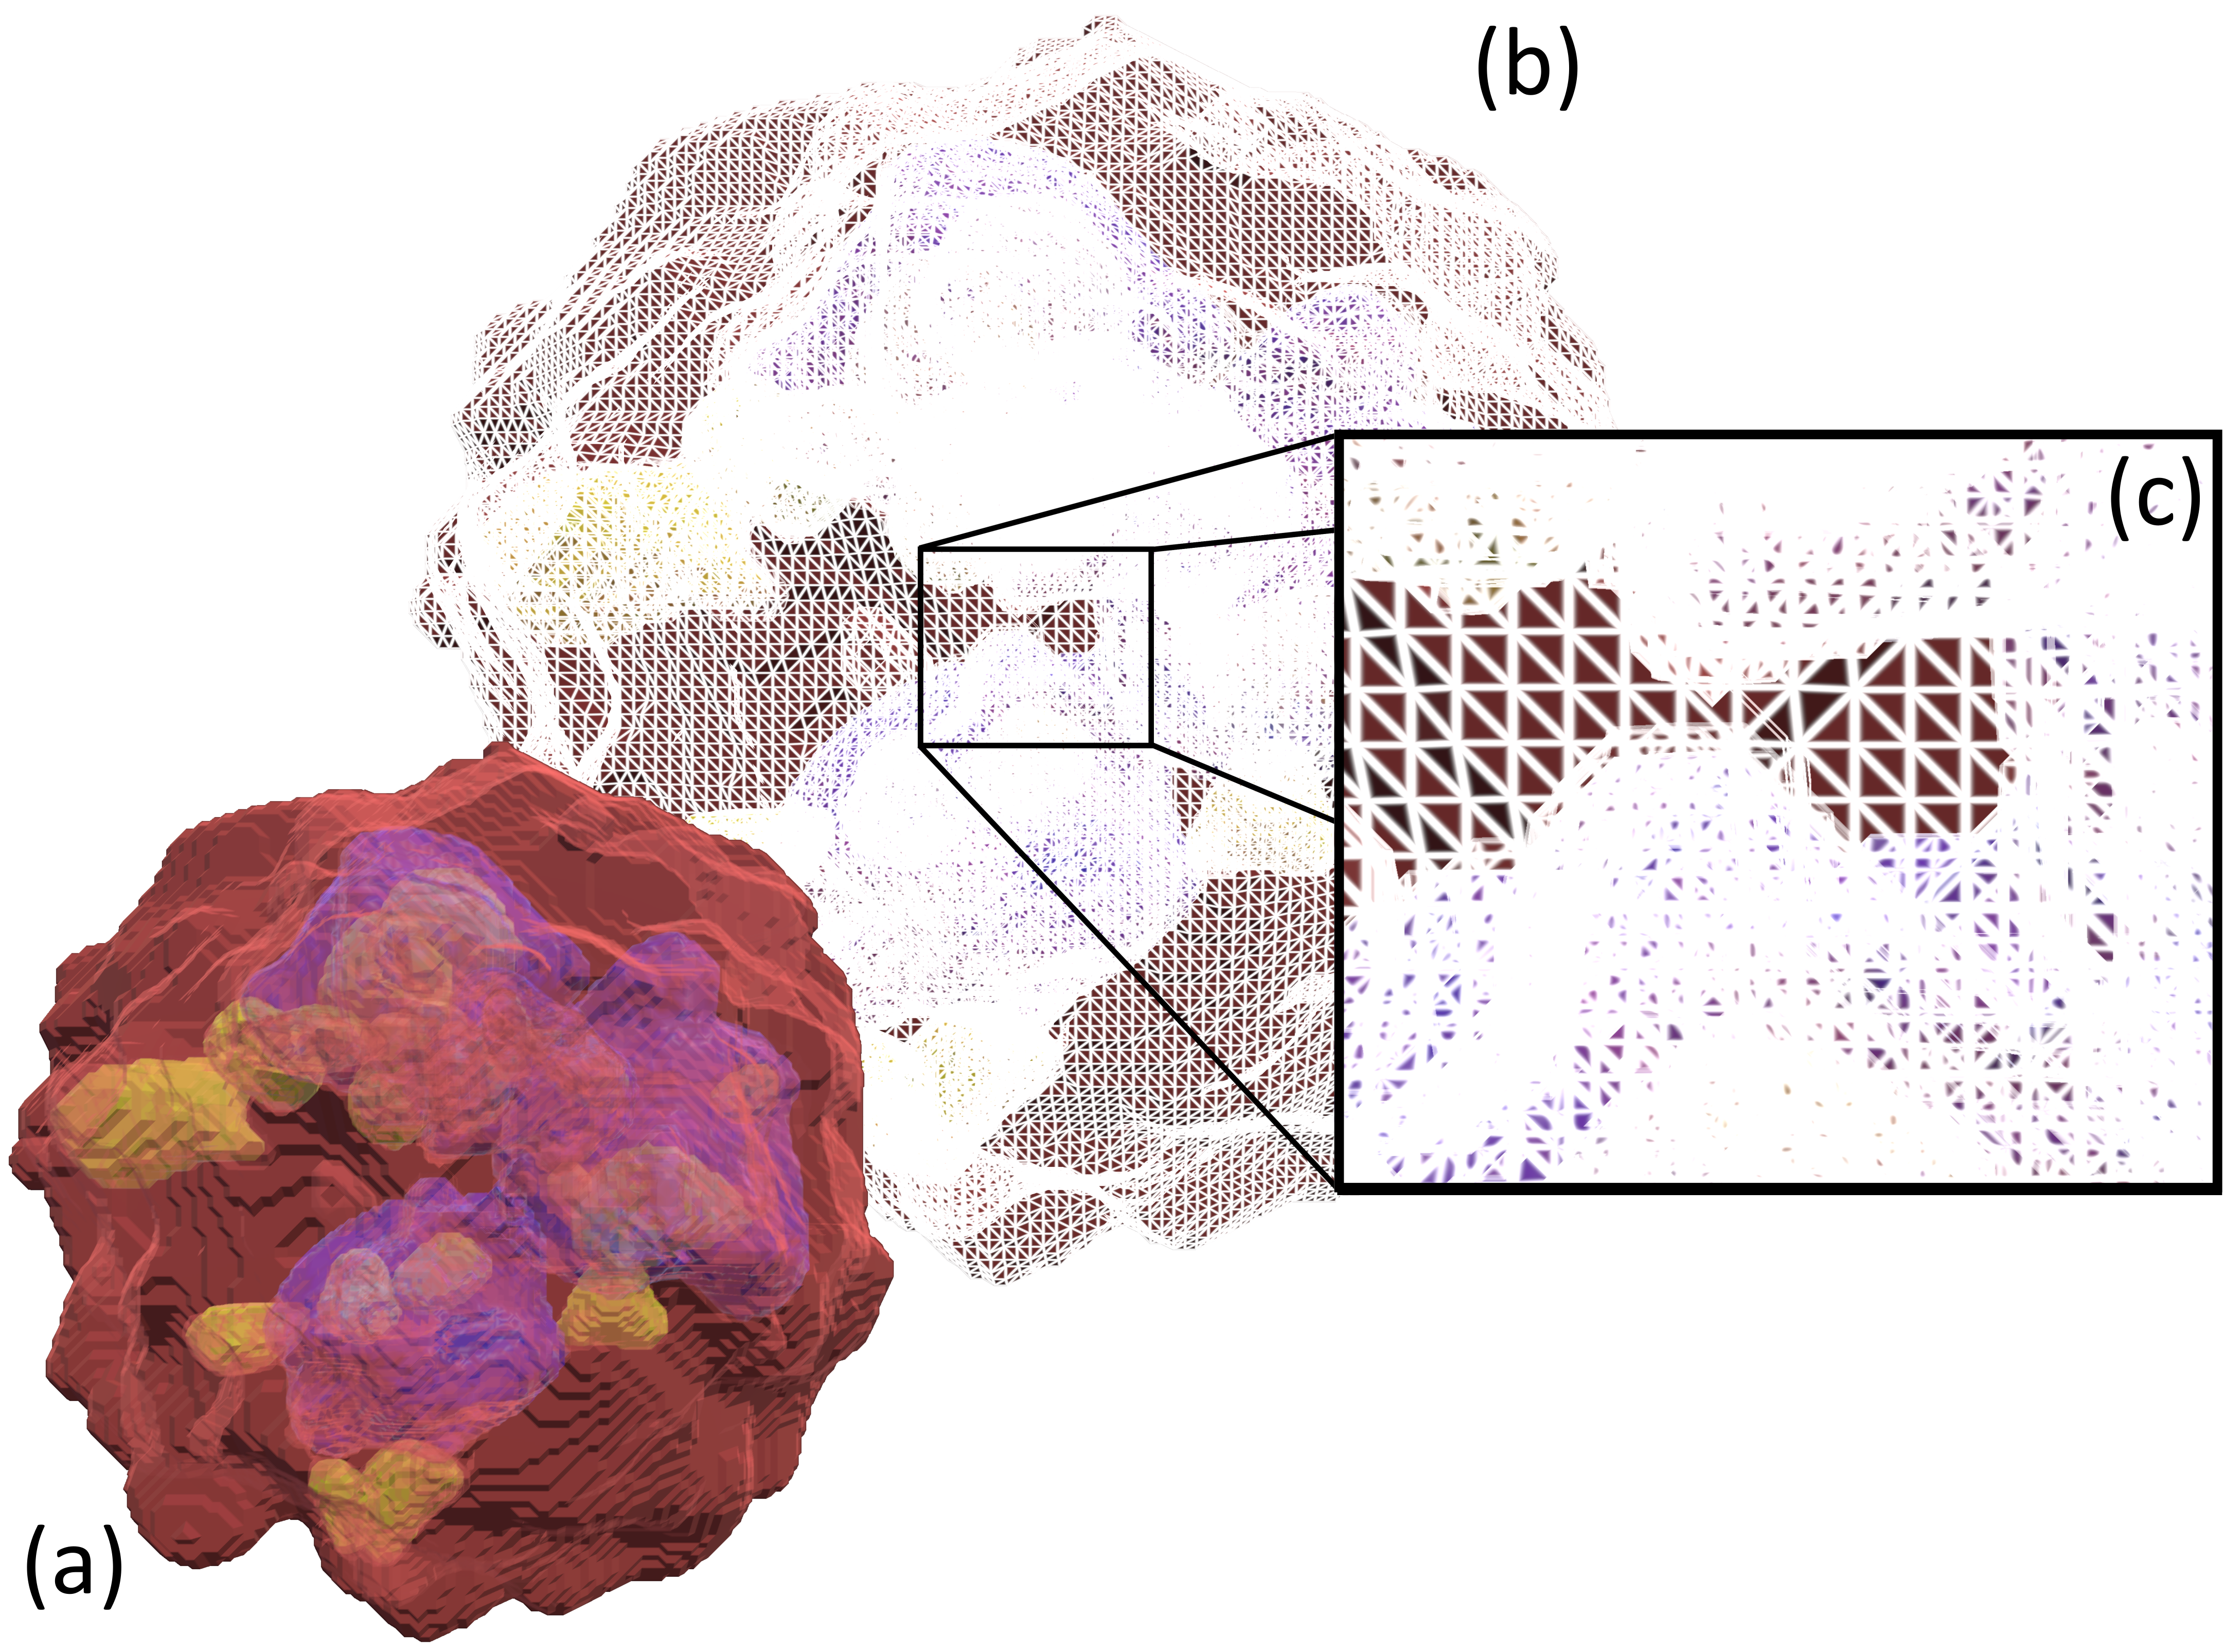
\includegraphics[width=\columnwidth]{Chapter4/Images/DiagramOfTheMeshes.png}
    \caption[A breakdown of the structures of the 3D meshes generated by the Random Volume Generator.]{A breakdown of the structures of the 3D meshes generated by the Random Volume Generator. a) presents the volume using transparent colors to show the different levels that meshes can be segmented, b) is the same volume but covered in a wireframe, c) is a close-up shot of the center b.}
    \label{fig:MeshVersionOfTheSystems}
\end{figure}

% 
The output from these files can provide mesh file outputs (.obj and .stl) or show DVR content in a JSON format.
The meshes are created via marching, running the iso-surface algorithm marching cubes~\cite{Lorensen} over the volume and can be created at any resolution required. 
The volume can be saved as a single mesh or a collection of smaller meshes (as shown in \autoref{fig:MeshVersionOfTheSystems}) spaced appropriately apart
allowing game engines and most displays to render them natively.
It can also create a 3D printable model (as seen in \autoref{fig:3DPrintedVersionOfTheSystem}).

The JSON file is designed to be read as input for a user study. 
It contains instructions on what condition the visualization was built for, the noise key, and any answers required for each volume, like volumetric information and the number of volumes contained under a certain circumstance. 
%This modular system can be redesigned for many DVR studies using Augmented Reality (AR) or Virtual Reality (VR) devices. 

\begin{figure}[bt]
    \centering
    \includegraphics[width=\columnwidth]{Chapter4/Images/3DPrintedObjectWithX-rayVision_ThesisVersion.png}
    \caption{(a) A 3D printed version of the model made from the Random Volume Generator's mesh output. (b and c) shows this model from the view of a Microsoft Hololens2 to create an \gls{X-ray Vision} effect using illustrative rendering.}
    \label{fig:3DPrintedVersionOfTheSystem}
\end{figure}

\subsection{Immersive User Interface Design} \label{sec:ImmersiveDesgin}
The Random Volume Generator's immersive design component is where the volumes are randomly generated while the user can change a set of parameters with the goal of creating an input file for the final system. 
By immersing researchers in the same environment as their users, they can experience the data set the same way their participants would while choosing parameters for various instances of the project.

The \gls{ui} elements have been generated from the Mixed Reality Tool Kit (MRTK)~\footnote{\url{https://github.com/microsoft/MixedRealityToolkit-Unity}} and have been laid out to keep the users focused on the volume. 
These elements include changing two list menus between a predefined set of conditions (this dissertation utilized \glspl{virt}) and updating input parameters (shown up the top and to the right of \autoref{fig:HoloLensInterface}).
All areas that can be modified via the selected parameters will be highlighted unless the "Custom Visualizations" option is enabled, showing the set of pre-computed visualizations that have been developed for the system.
Most of the input parameters users can be changed via to sliders (seen on the right side of \autoref{fig:HoloLensInterface}) that will allow them to choose between various sizes and amounts of objects that they want to exist at a time.

Since this interface exists in 3D, it is important to create a color interface that the interface suits this purpose. 
Unlike many color pickers used in \gls{vr}, which focus on a 2D input~\cite{Alex2020}, it was believed that this interface would benefit from giving the participants the ability to adjust the color with depth as of field as well. 
Requiring a volumetric color picker (shown down the bottom of \autoref{fig:HoloLensInterface}).
The colors for the elements of the volume can be chosen from a 3D color picker in a similar style to Kim et al.'s~\cite{Kim2022} color pickers designed for color blending.
% where direct volume rendering is used to identify an object's color.


The Random Volume Generator is available on GitHub.
The Random Volume Generation system~\footnote{\url{https://github.com/tomishninja/RandomlyGeneratingVolumes}} is built as a modular system built in the Unity game engine~\footnote{\url{https://unity.com/releases/editor/archive}}.

\section{Conclusion}

\begin{figure}[tb]
    \centering
    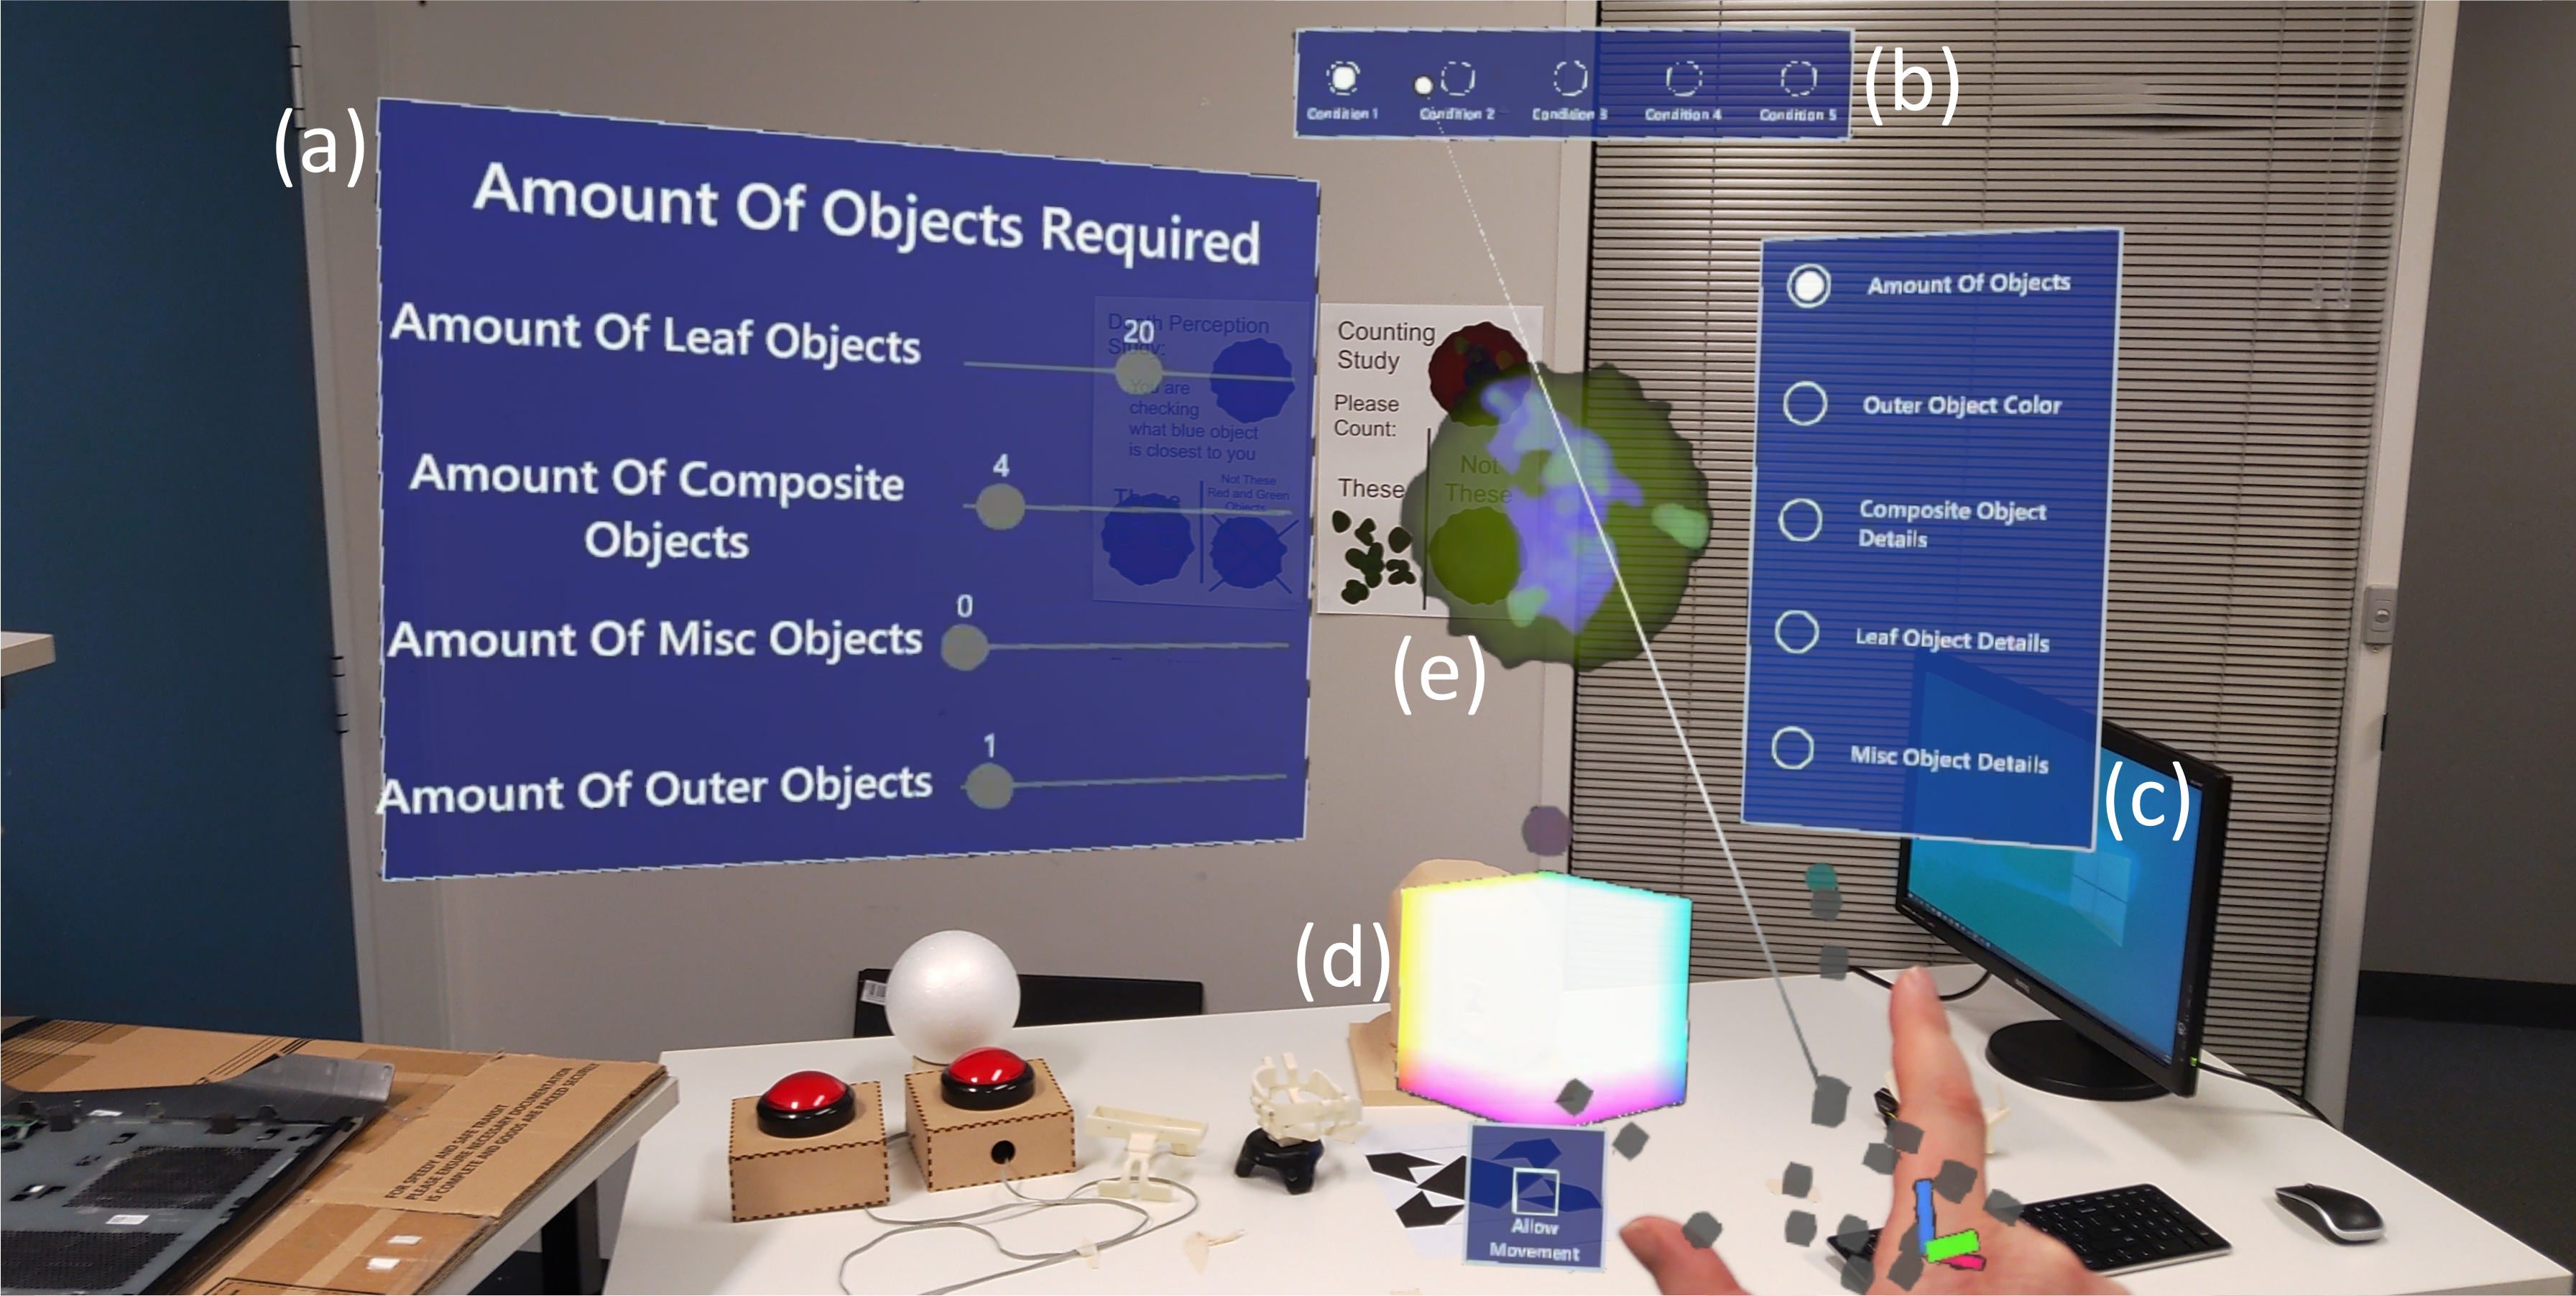
\includegraphics[width=\columnwidth]{Chapter4/Images/HoloLensTeaser.png}
    \caption{The HoloLens \gls{ui} of the random volume generation system. }
    \label{fig:HoloLensInterface}
\end{figure}

The Random Volume Generation System provides a method for generating volumes designed for different types of user studies that look into volumetric research in the 3D space. 
It provides a solution to the limited number of volumetric datasets that are available publicly and allows for more accurate results from controlled studies. 
This now lays the groundwork for future research to determine what \glspl{virt} the effects as \glspl{X-ray Visualization} have when used in tandem with \gls{dvr} utilizing a set of controls.
Moving forward, the goal is to test the perception and depth perception qualities of these visualizations on the general population by using these volumes with a series of tests designed to test the functionality of the \glspl{virt}. 

The Random Volume Generator provides researchers with:
\begin{itemize}
    \item A method for providing to recreate reproducible and a near-infinite amount of distinct volumes that can be easily transferred and stored for controlled studies. 
    \item An \gls{ar}/\gls{vr} interface to aid with the planning of these volumes.
    \item Open source access to the system and a guide to the modular components, which can be tailored for use with other studies.
\end{itemize}